\documentclass[main.tex]{subfiles}

\begin{document}
\section{Preliminary Test and Motivation}
The motivation for this work was to refine, understand, and document the \disp method of direction reconstruction. This method was expected to be useful to better resolve objects observed close to the horizon and facilitate studying the stability of the reconstruction to zenith angle of observation. There was also the possibility of using machine learning algorithms to improve resolution beyond that of the standard geometric reconstruction. In particular, an improved angular resolution on the Crab opens up the possibility of resolving the extension of the Crab Nebula with the VERITAS instrument.

A preliminary test for this was enabled by a set of runs where the Crab was tracked from horizon to culmination and back to the horizon (from the nights of Jan 12 2018, Jan 13 2018, and Jan 04, 2019). This provided a reference data set with high significance to track energy and zenith dependence of the direction reconstruction in stable (and therefore directly comparable) weather conditions. The differential resolution for the Crab data was measured in several energy and zenith bins and is presented in Fig. \ref{fig:crab_initial}

\begin{figure}[H]
  \begin{center}
    \subfigure[Crab reconstructed resolution using Method0.]{ 
      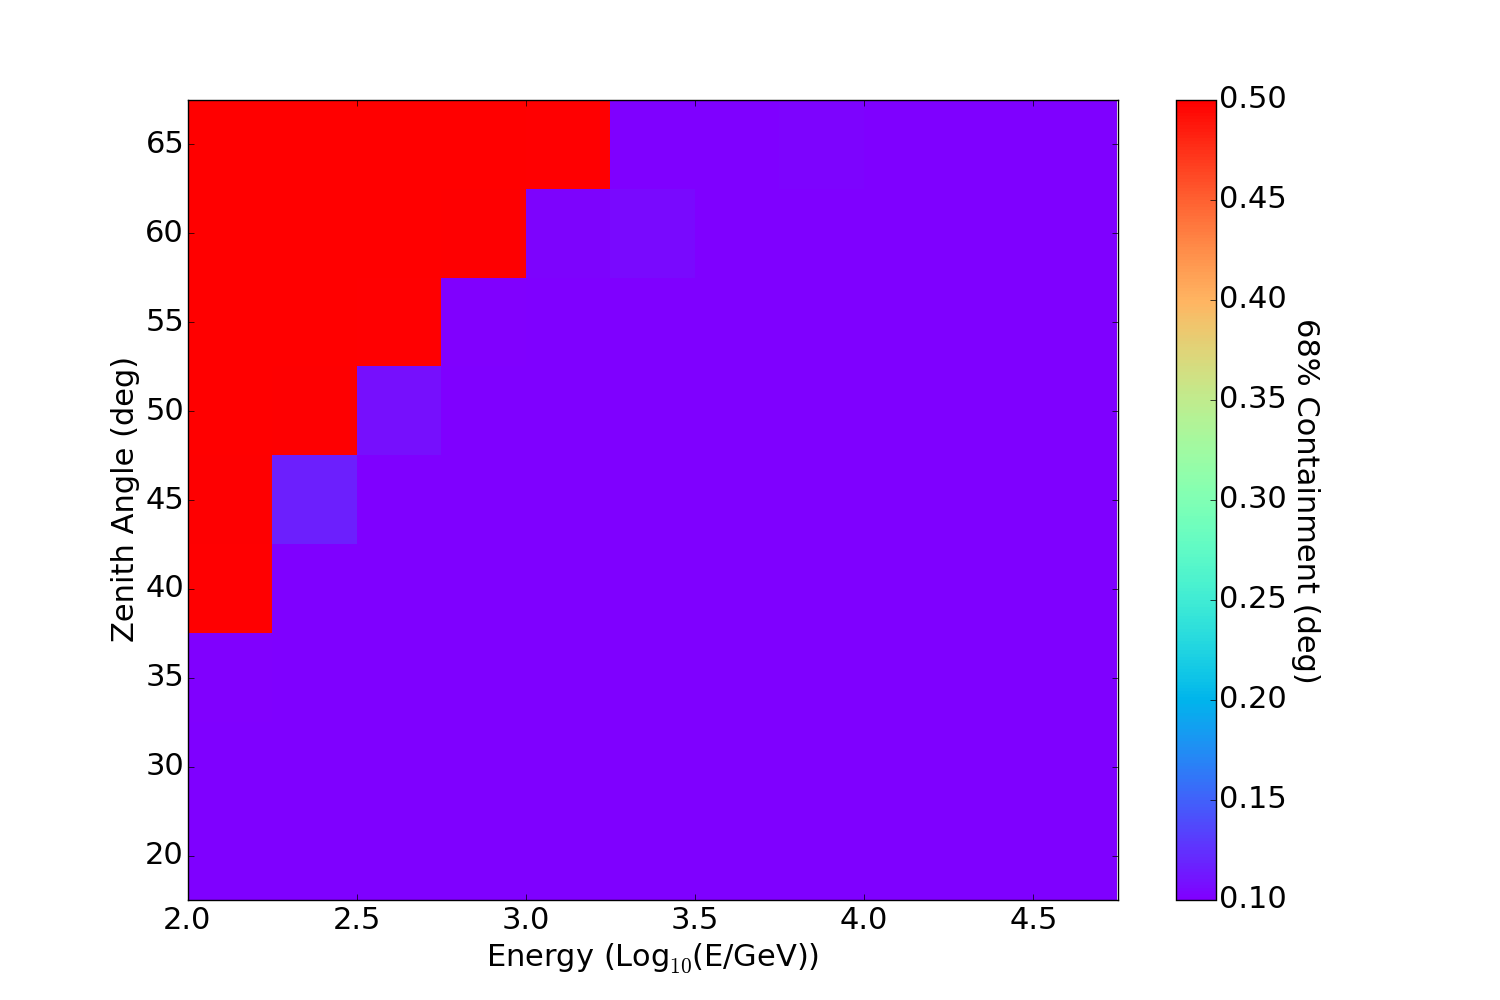
\includegraphics[width=0.47\linewidth]{crab_reg_rse.png}
      \label{fig:crab_reg_res}
    }  
    \subfigure[Crab binned significance.]{ 
      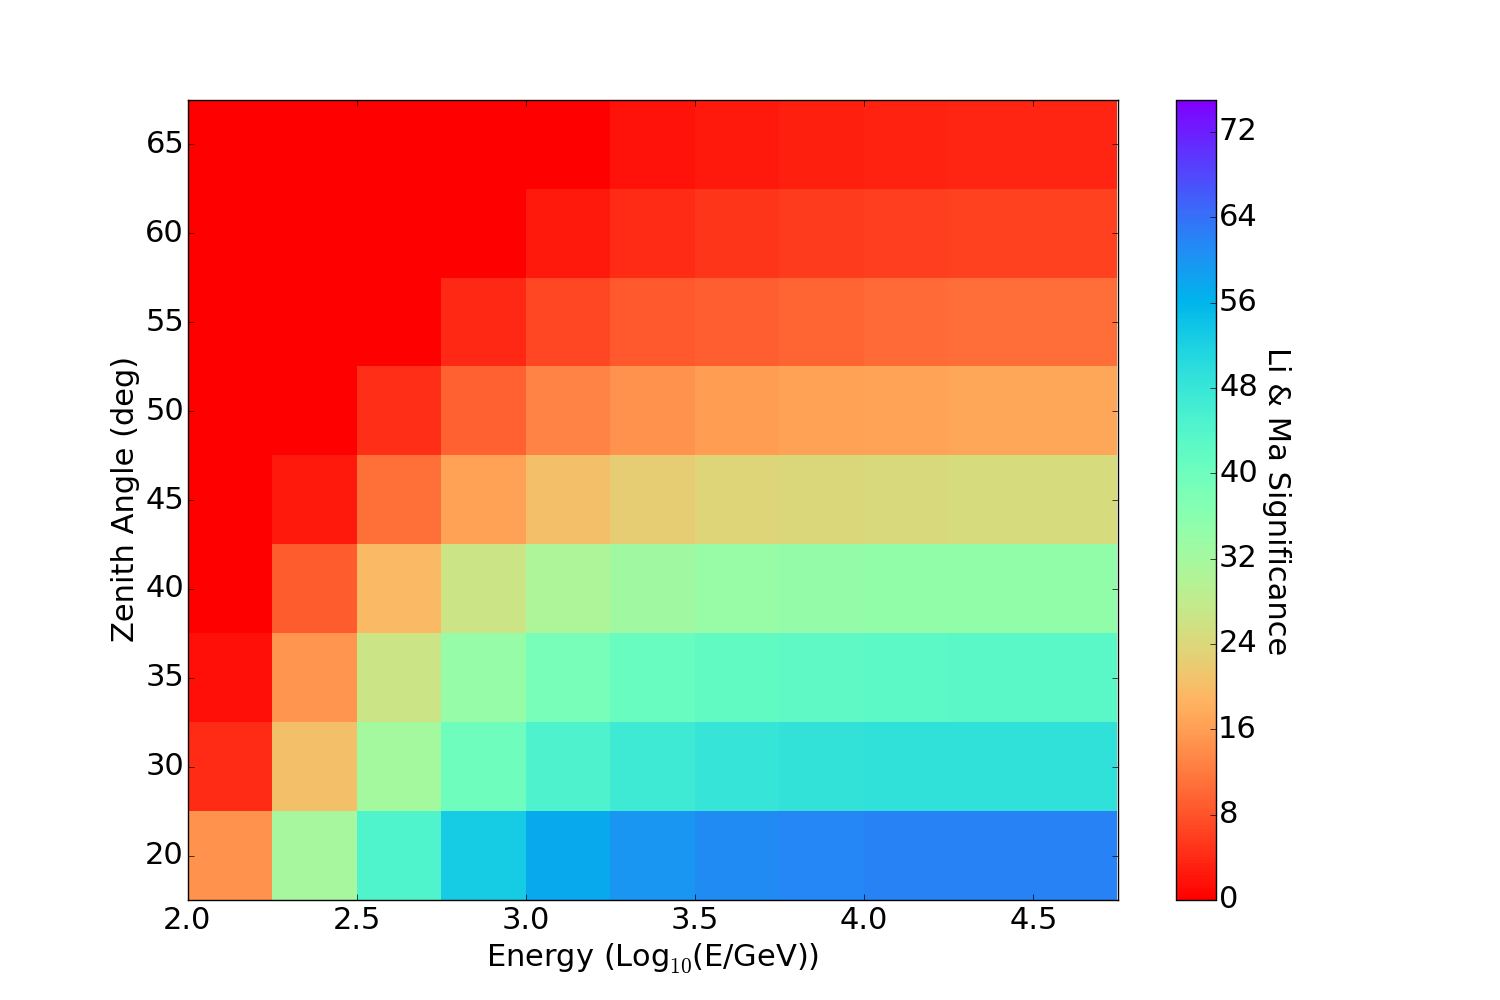
\includegraphics[width=0.47\linewidth]{crab_reg_LiMa.png}
      \label{fig:crab_res_num}
    }
  \end{center}
  \caption[Crab direction reconstruction using Method0.]{Reconstruction of the Crab direction using Method0 (standard geometric reconstruction from \textit{VEGAS}).}
  \label{fig:crab_initial}
\end{figure}

% The first part of this work was to examine the stability of the reconstructed Crab spectrum looking at the photon index and the integral flux above a threshold value based on the lowest energy where photons were reconstructed across zenith angles. The data used were from nights of horizon-to-horizon Crab runs (Jan 12 2018, Jan 13 2018, and Jan 04, 2019), where Crab runs were taken from the horizon to culmination and back to the horizon.

% For Method0, the reconstructed energy spectra appear to be largely stable under variations in zenith angle (Fig. \ref{fig:index_compare} and \ref{fig:intf_compare}). The slopes of the best fit gradient lines are insignificant for both the integral flux above the threshold energy ($10^{0.35} \approx 2.24$TeV) and the spectral index -- as they should be since physically these quantities are independent of zenith angle.

% The \disp method is able to reconstruct events down to larger zenith angles than the standard method although lower statistics at large zenith angles lead to larger uncertainties. However, the integral flux from the \disp method fit has a significant positive correlation with zenith angle, and lies significantly below the integral flux reconstructed from Method0.

% \begin{figure}[H]
%   \begin{center}
%     \subfigure[Crab reconstructed spectral index using Method0 and Method5t.]{ 
%       \includegraphics[width=0.9\linewidth]{images/Crab_C2C/Index_compare}
%       \label{fig:index_compare}
%     }  
%     \subfigure[Crab reconstructed integral flux above 2.24 TeV ($10^{0.35}$ TeV) using Method0 and Method5t.]{ 
%       \includegraphics[width=0.9\linewidth]{images/Crab_C2C/Intf_compare}
%       \label{fig:intf_compare}
%     }
%   \end{center}
%   \caption[Crab spectrum reconstruction.]{Reconstruction of the Crab spectrum using Method0 (standard reconstruction from \vegas) and Method5t (\disp).}
%   \label{fig:spectrum_compare}
% \end{figure}


\section{\disp Table and \rse Dependencies}
The BDT weight tables were generated independently of the old \disp method in order to have clear documentation of the underlying effects and dependencies. For the purposes of this work, the 68\% containment radius in angular offset (\rse\hspace{-4pt}) is used as a measure of angular resolution and performance of the reconstruction.

\subsection{Zenith Angle Dependence}
A set of \disp tables was generated with a small sample of events ($n\approx 1.9\e6$) across the range of zenith angles of interest ($20^\circ-65^\circ$). This was compared to the regular \disp method. Since there was no record of the training sample size for the standard tables, this test sample was useful in determining the resolution of the \disp method with a relatively small computational footprint. Additionally, it allowed for some simple tests of dependence of the \disp tables on parameters not explicitly in the \disp tables.

This small \disp tables and the standard \disp tables were used to reconstruct simulation events and compared with Method0 (the standard method of direction reconstruction). In both cases, the \disp method performs better than Method0 at the largest zenith angles ($\geq 55^\circ$, see \ref{fig:olddisp_ratio}-\ref{fig:disp_ratio_250} for \rse of the \disp methods divided by that for Method0 at the same zenith angle). From here it is clear that the regime of interest for the \disp method is $\geq45^\circ$. 

\begin{figure}[htbp]
  \begin{center}
      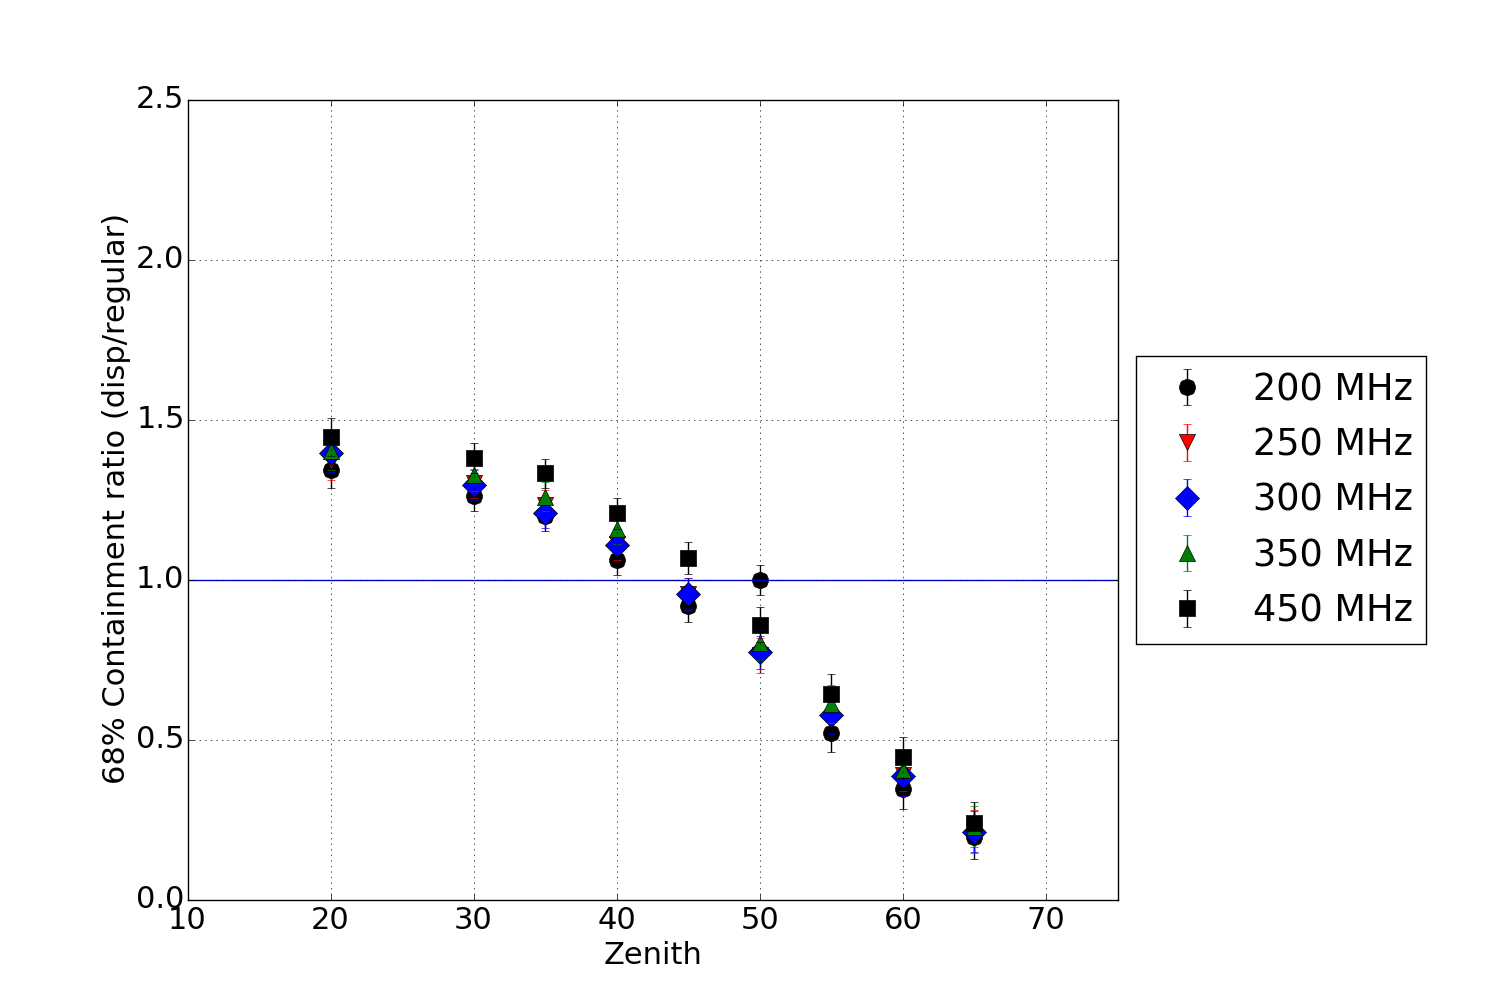
\includegraphics[width=0.75\linewidth]{images/disp_standard_ratio_xzen}
      \caption[``standard'' \disp table reconstruction.]{Ratio of \rse of the ``standard'' \disp table to that from Method0. Since this is the ratio of methods, the horizontal blue line denotes the performance using Method0, and this method performs better than Method0 for zenith $>45^\circ$.}  
      \label{fig:olddisp_ratio}
  \end{center}
\end{figure}

\begin{figure}[htbp]
  \centering
  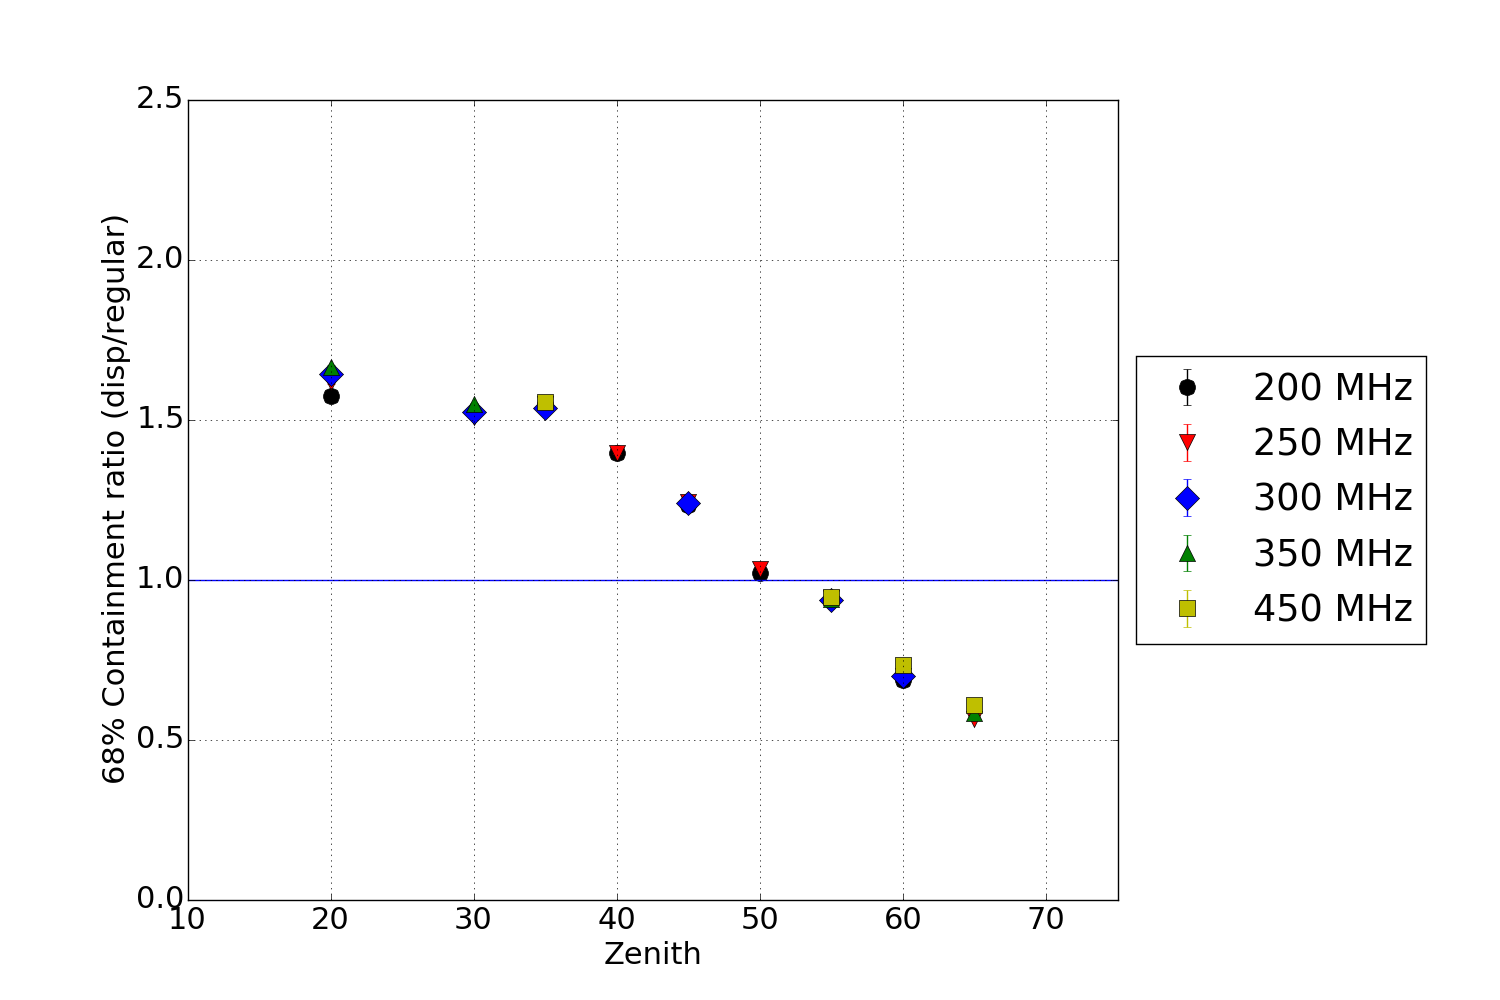
\includegraphics[width=0.75\linewidth]{images/disp_250_ratio_xzen}
  \caption[Small \disp table reconstruction (noise = $250$ MHz).]{Ratio of the \rse from reconstruction using the small \disp table ($\sim 1.9\e6$ events all at noise $= 250$ MHz) and that from Method0. Note the horizontal blue line denotes the performance using Method0, so this method performs better than Method0 for zenith $>45^\circ$.}
  \label{fig:disp_ratio_250}
\end{figure}

\subsection{Over-training}
BDT based regression is quite robust under non-linear correlations between discriminating parameters, however the primary vulnerability of this method, is that  to over-training - where the decision tree starts to be informed by noise and nuisance parameters in the training sample rather than relevant effects. This results in substantially different reconstruction efficiencies between training and testing samples. The ROOT TMVA package has a built-in test for over-training where it randomly selects a given fraction of the supplied events (for the purposes of this work, this fraction was taken to be 50\%) to use for testing. These events are then not used to train the regression trees and are instead used only to generate a measure of the over-training.
This check of the over-training for one of the test tables (noise $= 450$ MHz), shown in Fig. \ref{fig:overtraining}, demonstrates that there was no meaningful over-training of the table at least based on effects in the training sample.

There remains however, the possibility of effects related to noise level that might appear in the training \textit{and} testing samples (which are generated separately at each noise level), but not in observational data sets, which would be overlooked by this measure of over-training.

\begin{figure}[H]
  \centering
  \subfigure[Deviation of reconstructed \disp parameter from Monte-Carlo \disp parameter in training sample.]{
    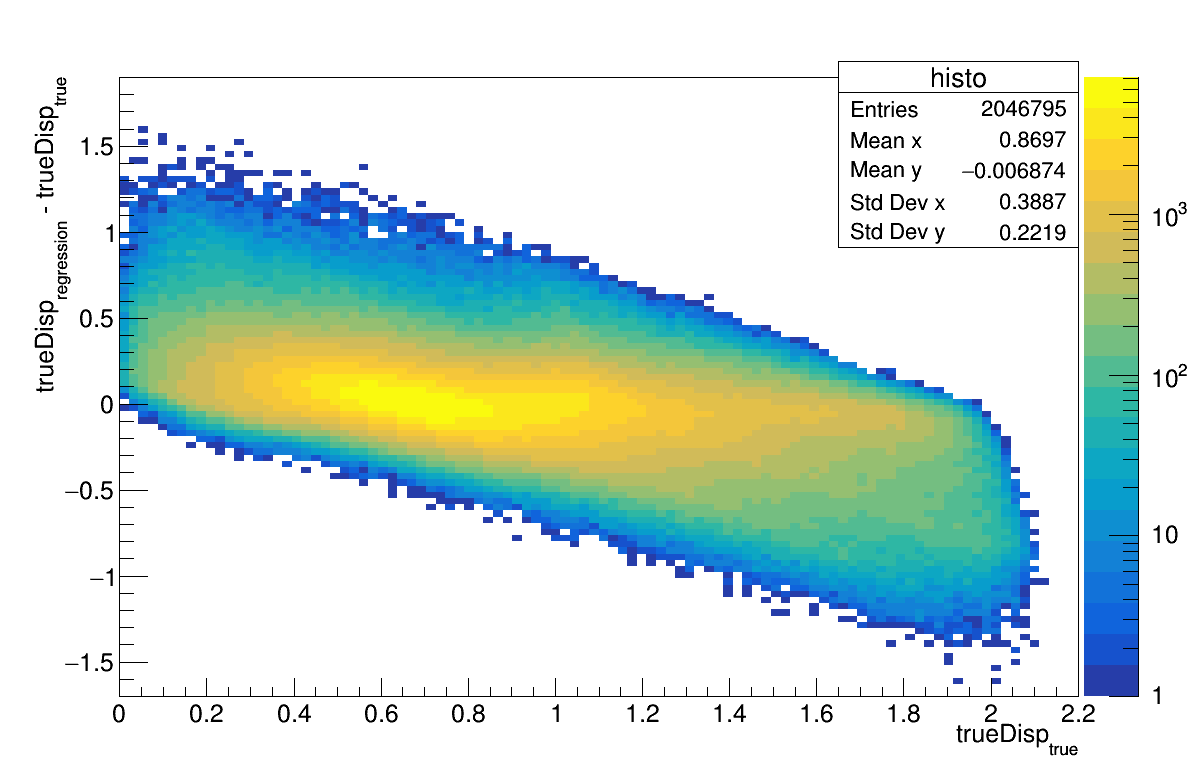
\includegraphics[width=.47\linewidth]{images/trueDisp_Train}
    \label{fig:disp_train_overtraining}
  }
  \subfigure[Deviation of reconstructed \disp parameter from Monte-Carlo \disp parameter in testing sample.]{
    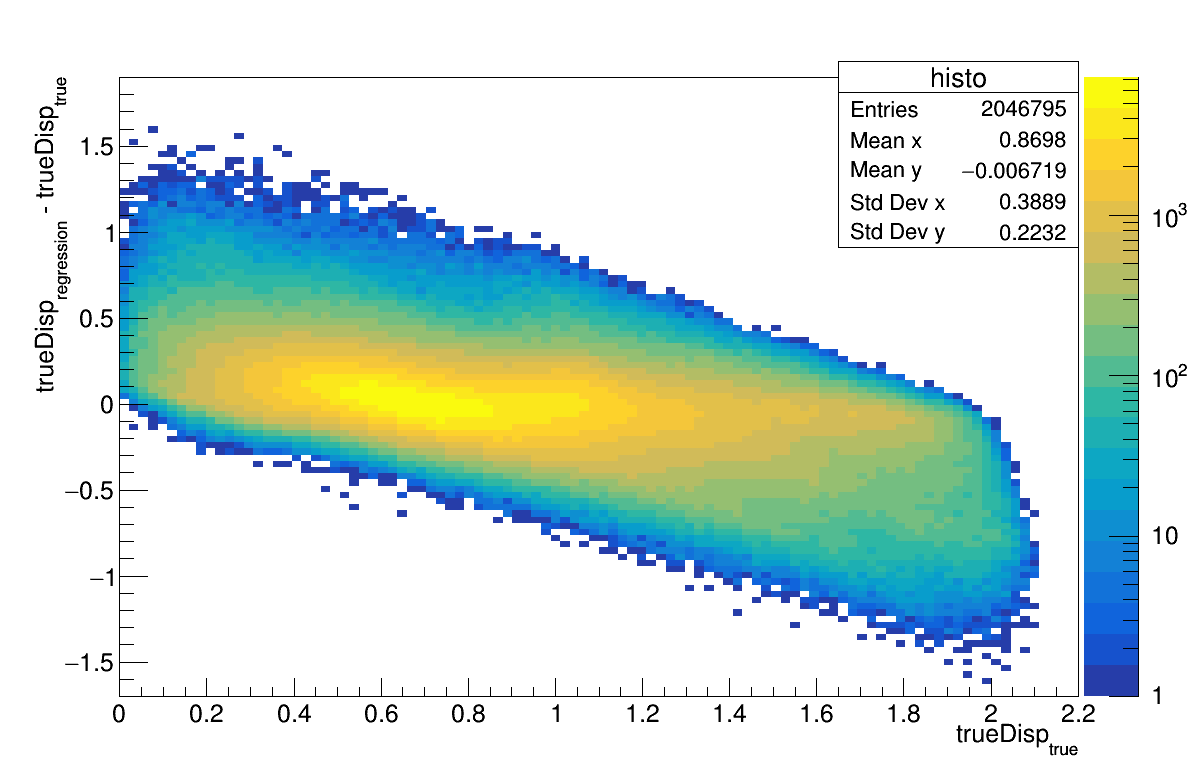
\includegraphics[width=.47\linewidth]{images/trueDisp_Test}
    \label{fig:disp_test_overtraining}
  }
  \subfigure[Deviation of reconstructed \disp Error parameter from Monte-Carlo \disp Error parameter in training sample.]{
    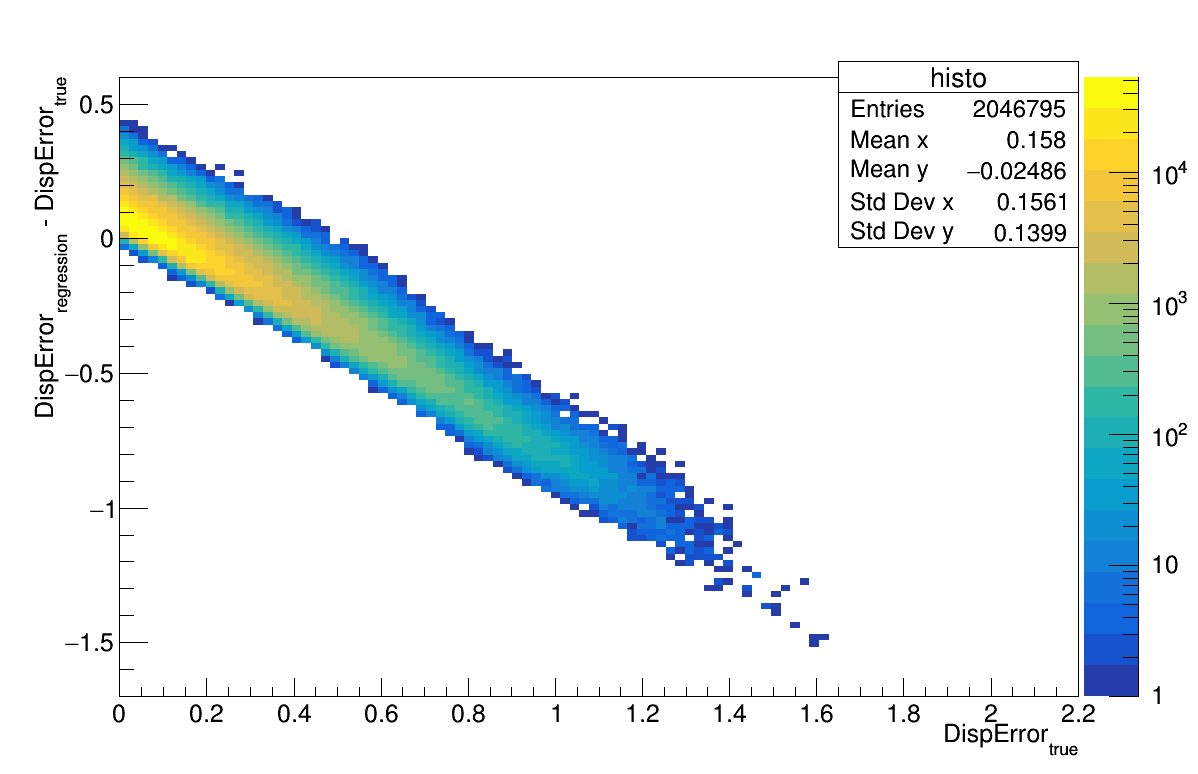
\includegraphics[width=.47\linewidth]{images/DispError_Train}
    \label{fig:dispErr_train_overtraining}
  }
  \subfigure[Deviation of reconstructed \disp Error parameter from Monte-Carlo \disp Error parameter in testing sample.]{
    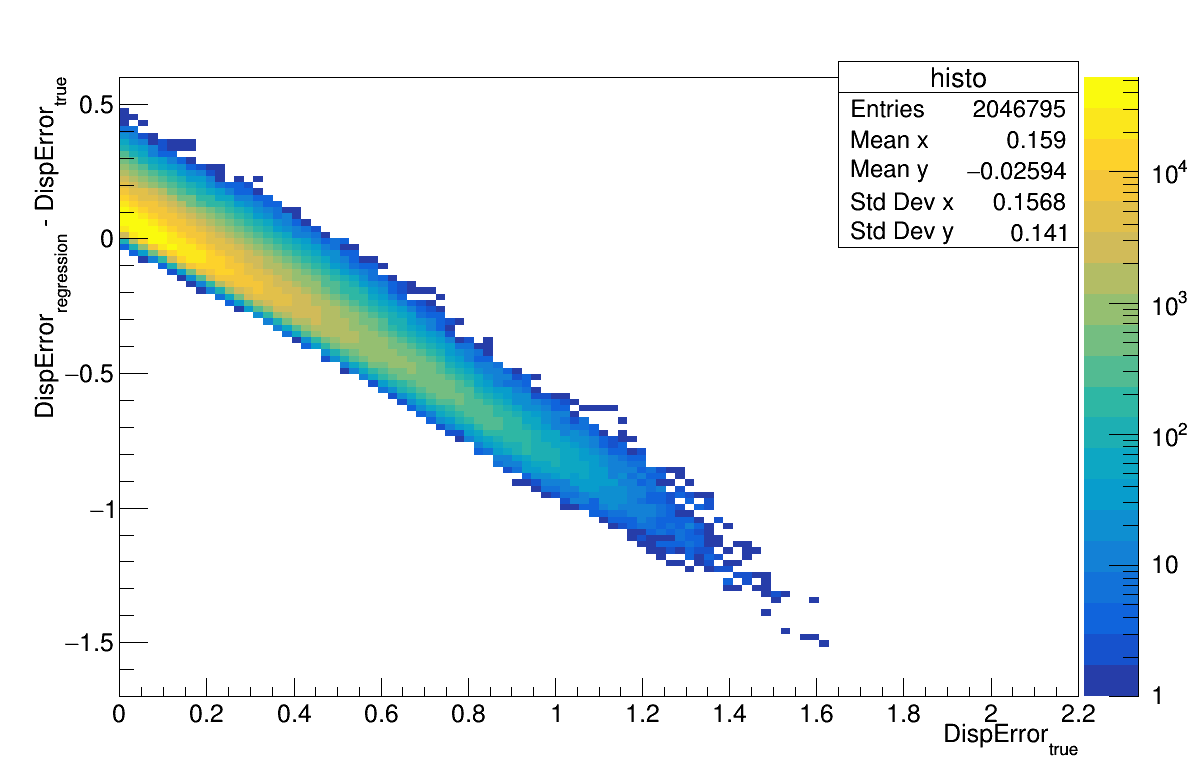
\includegraphics[width=.47\linewidth]{images/DispError_Test}
    \label{fig:dispErr_test_overtraining}
  }
  \subfigure[Deviation of reconstructed MAError parameter from Monte-Carlo MAError parameter in training sample.]{
    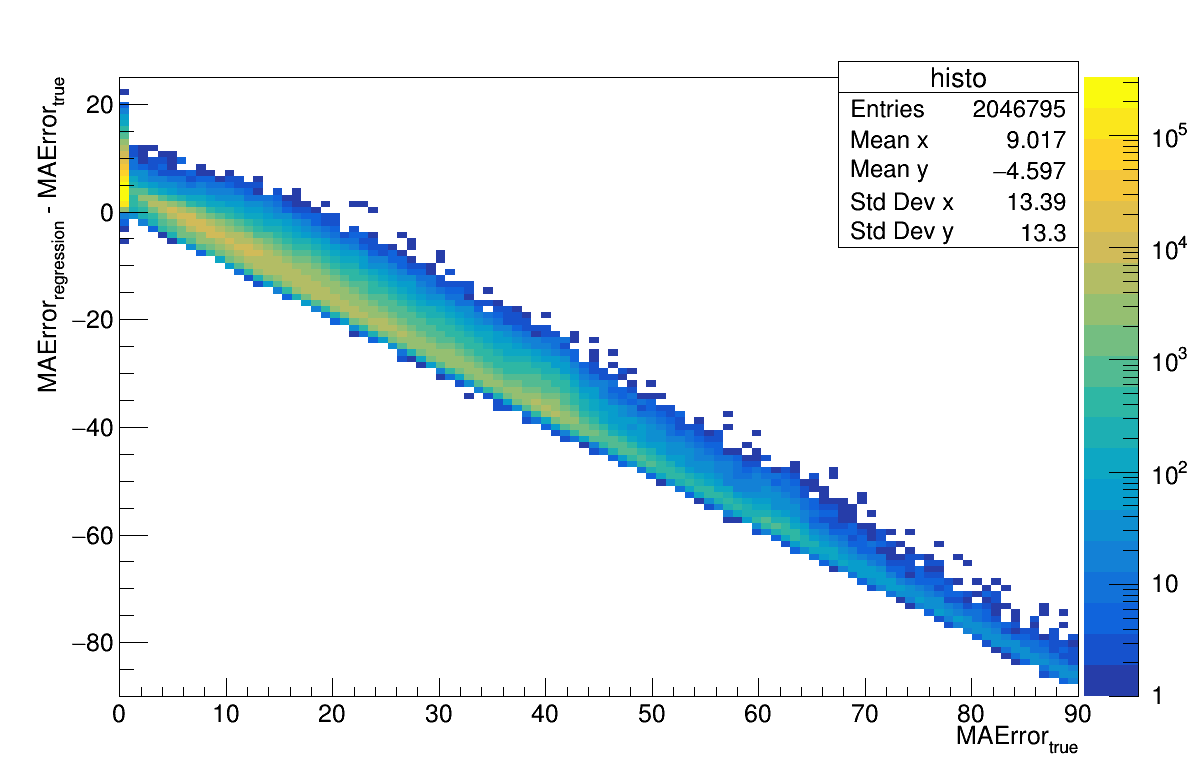
\includegraphics[width=.47\linewidth]{images/MAError_Train}
    \label{fig:MAErr_train_overtraining}
  }
  \subfigure[Deviation of reconstructed MAError parameter from Monte-Carlo MAError parameter in testing sample.]{
    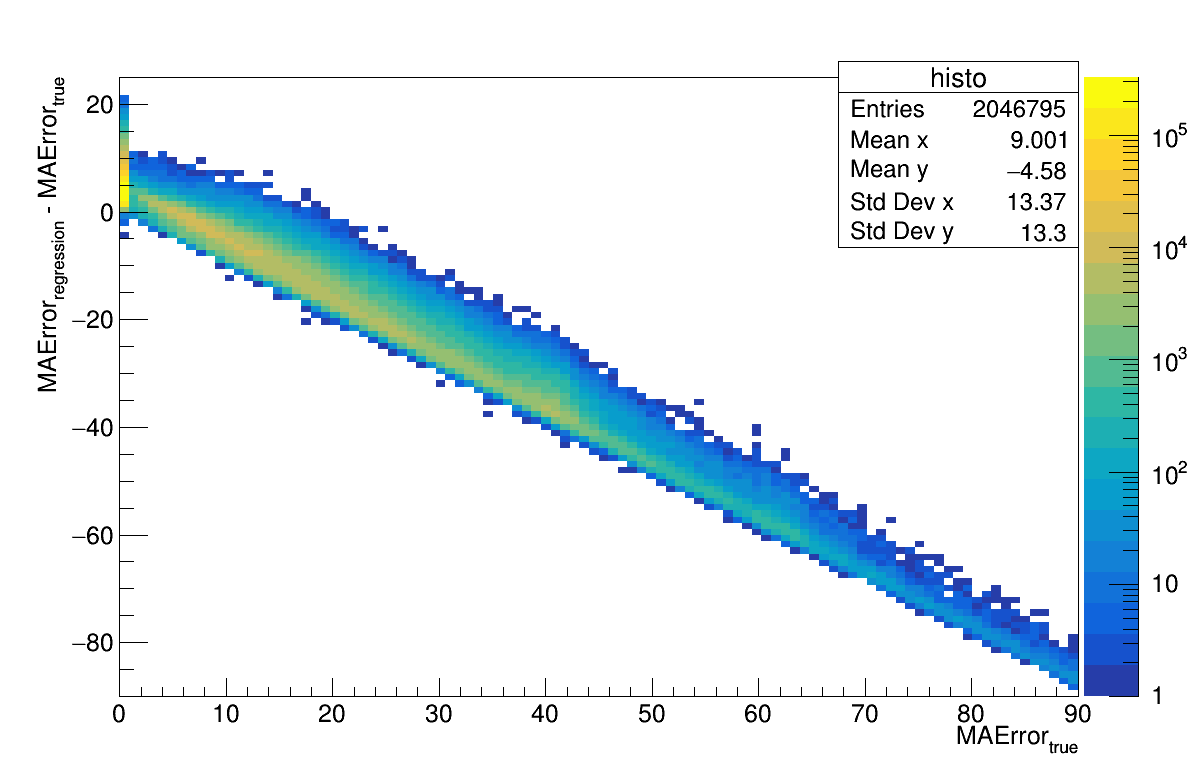
\includegraphics[width=.47\linewidth]{images/MAError_Test}
    \label{fig:MAErr_test_overtraining}
  }
  \caption[Over-training test.]{Over-training check on reconstruction using a \disp table generated at a single noise level. The left column shows the deviation of the reconstructed parameter from the true value in the training sample and the column on the right shows the same in the testing sample. The difference between the two columns is small which suggests there is little or no overtraining.}
  \label{fig:overtraining}
\end{figure}

\subsection{Noise Related Effects}
The first set of \disp tables was also generated at a single noise level ($250$ MHz), allowing us to test the dependence of the resolution of this method (as measured by R$_{68}$) on noise level -- some kind of noise-dependent effect would suggest over-training that would not be evident from the testing sample in the ROOT TMVA method since all the data provided to the package would have been at the same noise level. A comparison of angular resolution across noise levels revealed no significant dependence of the \rse on noise (see Fig. \ref{fig:olddisp_ratio}, \ref{fig:disp_ratio_250} and \ref{fig:disp_ratio_450}).

\begin{figure}[htbp]
  \centering
  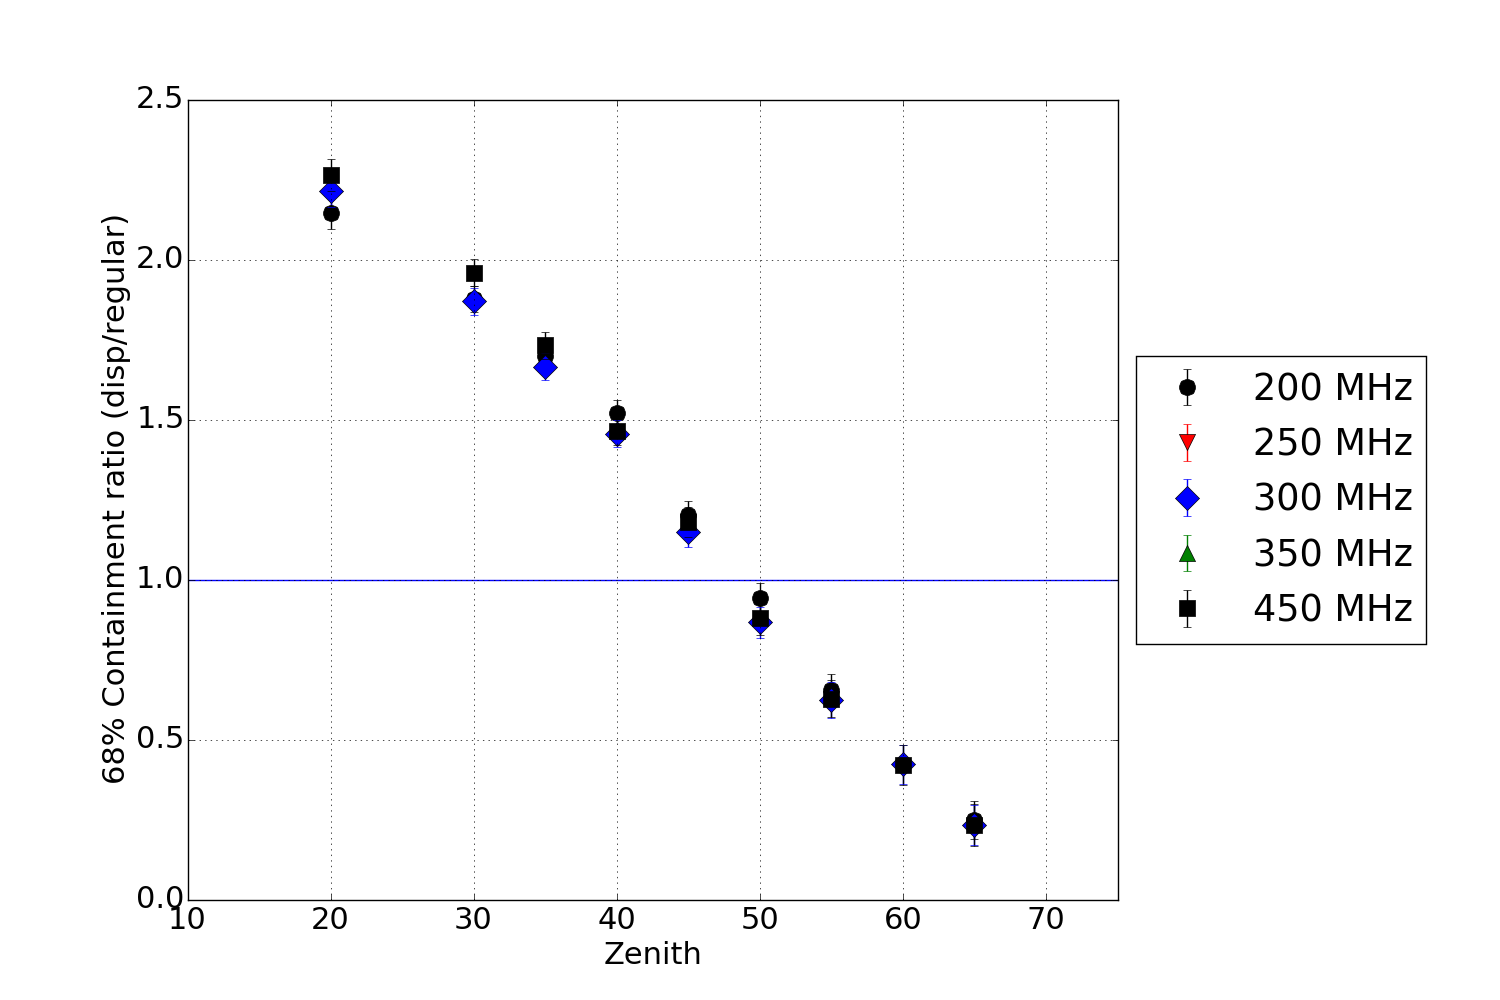
\includegraphics[width=0.8\linewidth]{images/disp_450_ratio_xzen}
  \caption[\disp table reconstruction vs noise.]{Ratio of \rse of the noise=450MHz \disp table ($\sim 2.1\e6$ events) to that from Method0.}
  \label{fig:disp_ratio_450}
\end{figure}

A second set of test \disp tables was generated using a single noise level (noise $= 450$ MHz) to test for noise-related over-training (see Fig. \ref{fig:disp_ratio_450}). These tables performed slightly better than the first test tables and comparably to the standard \disp tables. Since the noise-related effects did not seem to play a significant role in reconstruction, noise was dropped as a discriminating parameter for further analysis.

To generate a set of \disp tables with better angular resolution (as measured by \rse\hspace{-4pt}), another set of \disp tables was trained on a larger number of simulations across zenith angles (as before) as well as across the noise spectrum.

\subsection{Higher Statistics Tables}
Once it was determined that there was no significant over-training in the small sample \disp tables, and the noise level had little bearing on the \rse measure of the reconstruction, it was determined that different noise level simulation events could be used as independent training events to have a higher statistics \disp table, and make small improvements on the statistical uncertainty on the reconstruction. The simulation data from across the noise spectrum and zenith range was used to generate a \disp table that sampled the entire parameter space more exhaustively.

A new set of \disp tables was generated (Fig. \ref{fig:disp_ratio_450x4}) with a training sample four times that of the initial test tables. The improvements in resolution due to change in sample size were modest, and confined to the range of zenith angles (zenith $>45^\circ$) where the standard method outperforms the \disp method quite considerably.

\begin{figure}[htbp]
  \centering
  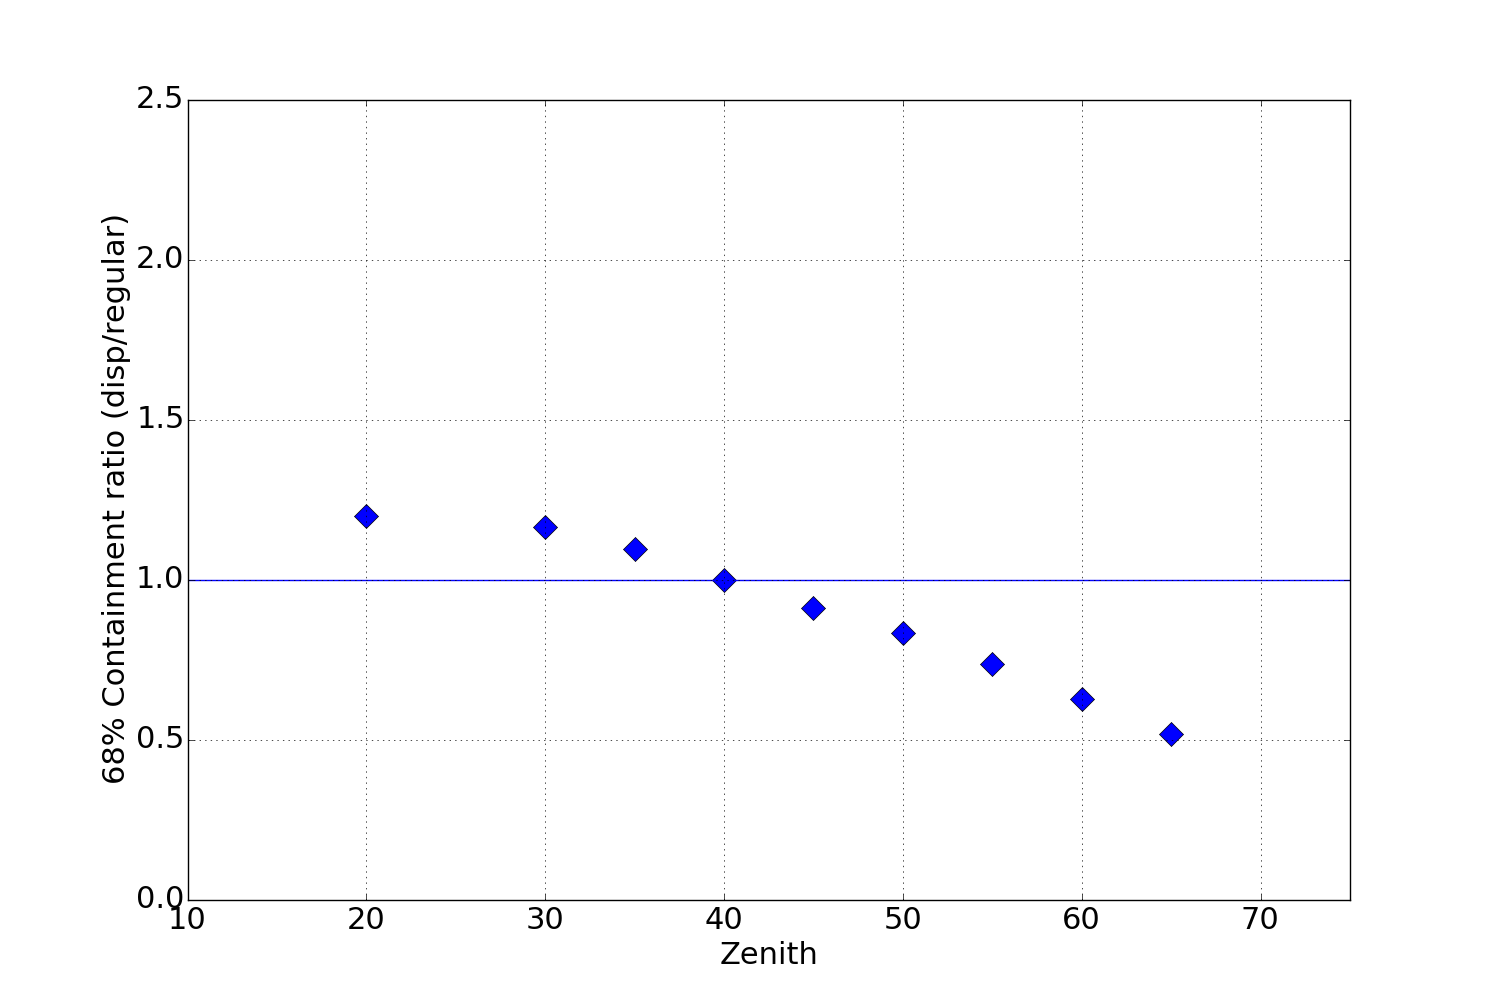
\includegraphics[width=0.8\linewidth]{images/disp_450x4size_ratio_xzen}
  \caption[Higher statistics \disp table reconstruction vs noise.]{Ratio of \rse of the noise=450MHz \disp table ($\sim 8.4\e6$ events) to that from Method0 for a higher statistics \disp table.}
  \label{fig:disp_ratio_450x4}
\end{figure}

As expected from the small statistical uncertainty on the \rse values, this increase in sample size did not lead to any meaningful improvements and a training sample of $\sim 2\e6$ was determined to be sufficient to achieve the desired resolution with small uncertainties.

\subsection{Acceptance Correction for Offset from Camera Center}
Showers arriving further from the camera center have a larger fraction of the shower arriving outside of the camera and therefore being lost. These showers are therefore reconstructed with a lower efficiency and resolution than showers arriving closer to the camera center. To compensate for this in the BDT training, so that the training sample does not mis-characterize the overabundance of events closer to the camera center as an anisotropy in incoming gamma rays, we fold in an acceptance correction by assigning a larger weight to events that are further away from the camera center.

The acceptance correction used here affects the training sample and therefore might be assumed to affect the resolution in a zenith dependent way, explaining the difference in performance between the new \disp tables and the old ones. This was tested by using a number of different correction functions in the training sample, as shown in Fig. \ref{fig:weights}

\begin{figure}[htbp]
  \centering
  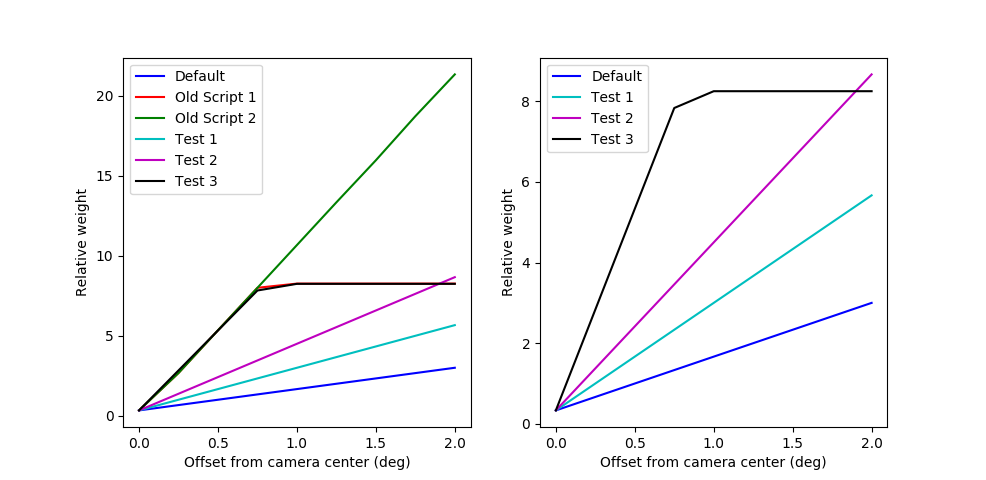
\includegraphics[width=.78\linewidth]{images/weights}
  \caption[Weight functions for offset from camera center.]{The weight functions used in the training samples in the new tables (Default, Test 1, Test 2 and Test 3) and those found in the scripts used to generate the older tables (Old Script 1, Old Script 2).}
  \label{fig:weights}
\end{figure}

These tests reveal small changes in the \rse value despite large changes in the correction function (Fig. \ref{fig:weight_tests}). This suggests that the \disp tables are not sensitive to changes in acceptance and therefore the different acceptance functions are unlikely to be the reason why the new \disp tables perform worse at smaller zenith angles.

\begin{figure}[htbp]
  \centering
  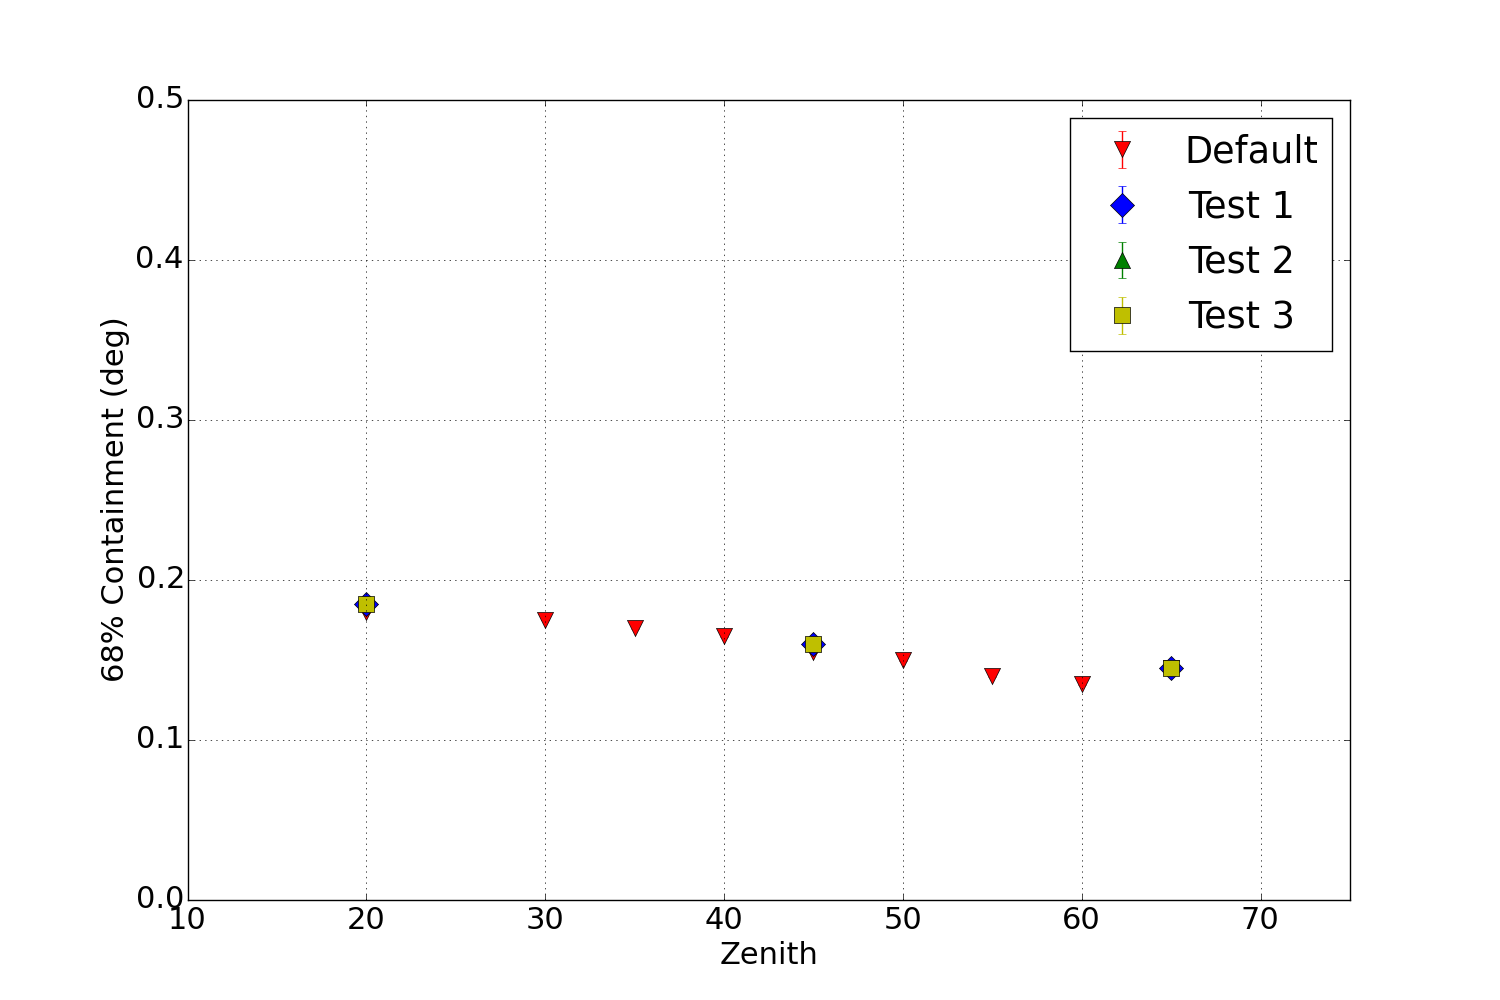
\includegraphics[width=.75\linewidth]{images/disp_wts_val_xzen}
  \caption[\rse for the acceptance correction functions.]{\rse for each acceptance correction function shown in Fig. \ref{fig:weights}. The changes in acceptance correction do not meaningfully change the \rse for the reconstruction.}
  \label{fig:weight_tests}
\end{figure}

\subsection{Energy Dependence}
Another important dependence of the reconstruction resolution (and therefore the R$_{68}$) is that on energy. Higher energy photons are expected to comprise a large fraction of LZA photons since they have to travel longer through the atmosphere and therefore must have higher energies to remain above the energy threshold. Conversely, high energy photons make up a small fraction of SZA photons (and more generally, all cosmic photons) due to the $\sim E^{-2}$ shape of the spectrum. A better resolution at higher energy would also be expected to contribute to the improved resolution at LZA.

\begin{figure}[htbp]
  \centering
  \subfigure[Energy Dependence of Method0 at small and medium zenith angles.]{
    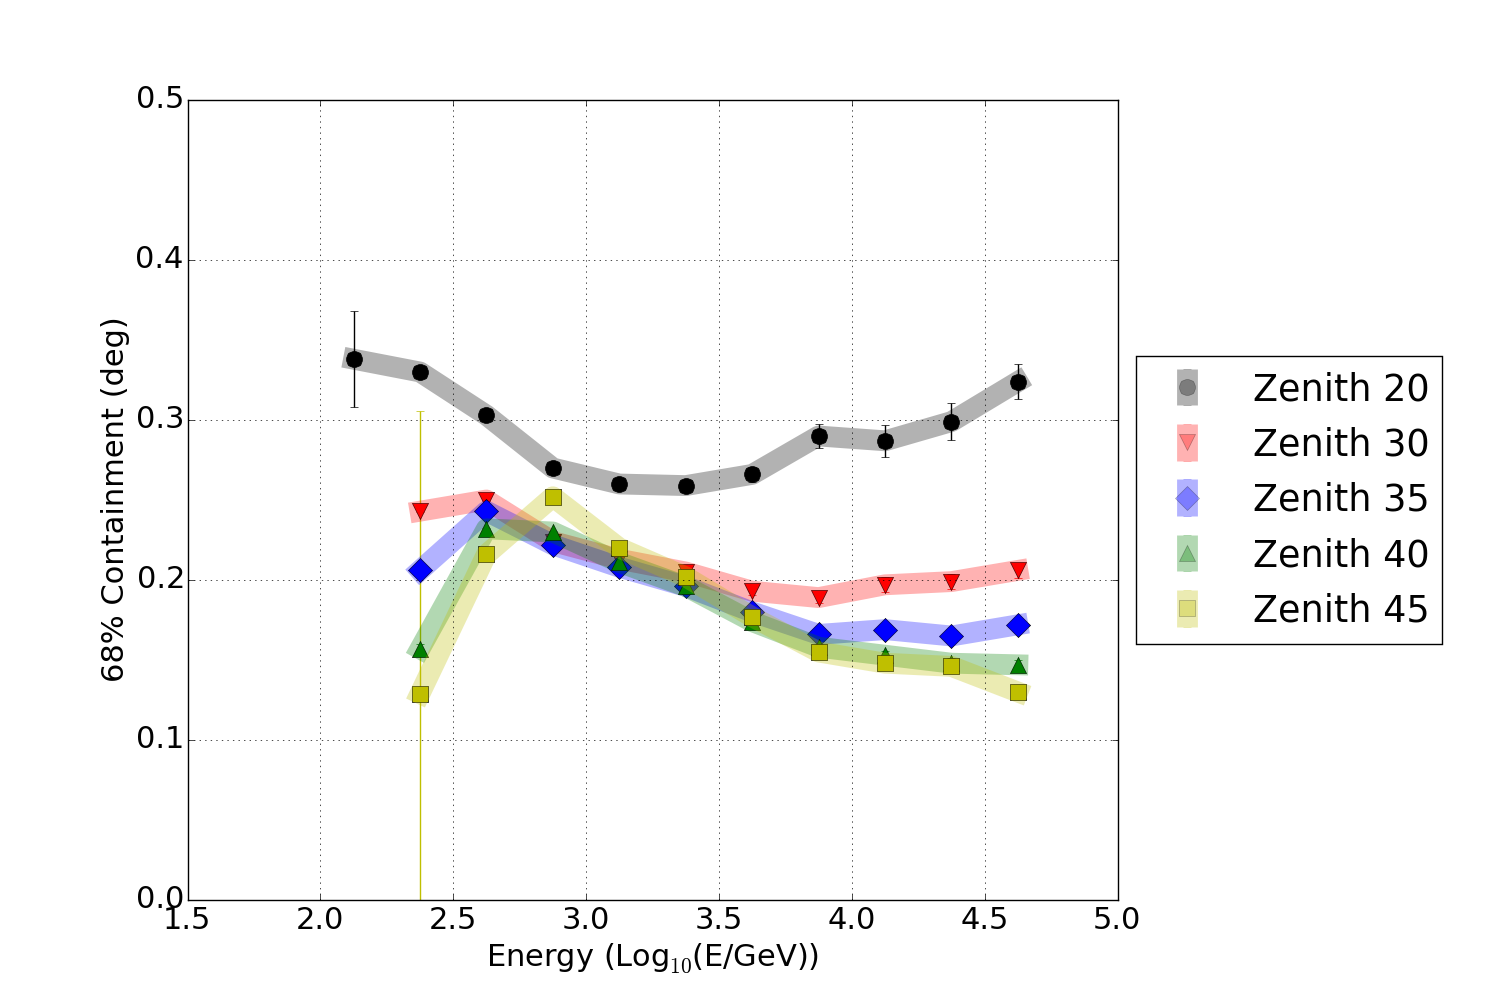
\includegraphics[width=.44\linewidth]{images/reg_energy_SZA}
    \label{fig:energy_reg_SZA}
  }
  \subfigure[Energy Dependence of Method0 at large zenith angles.]{
    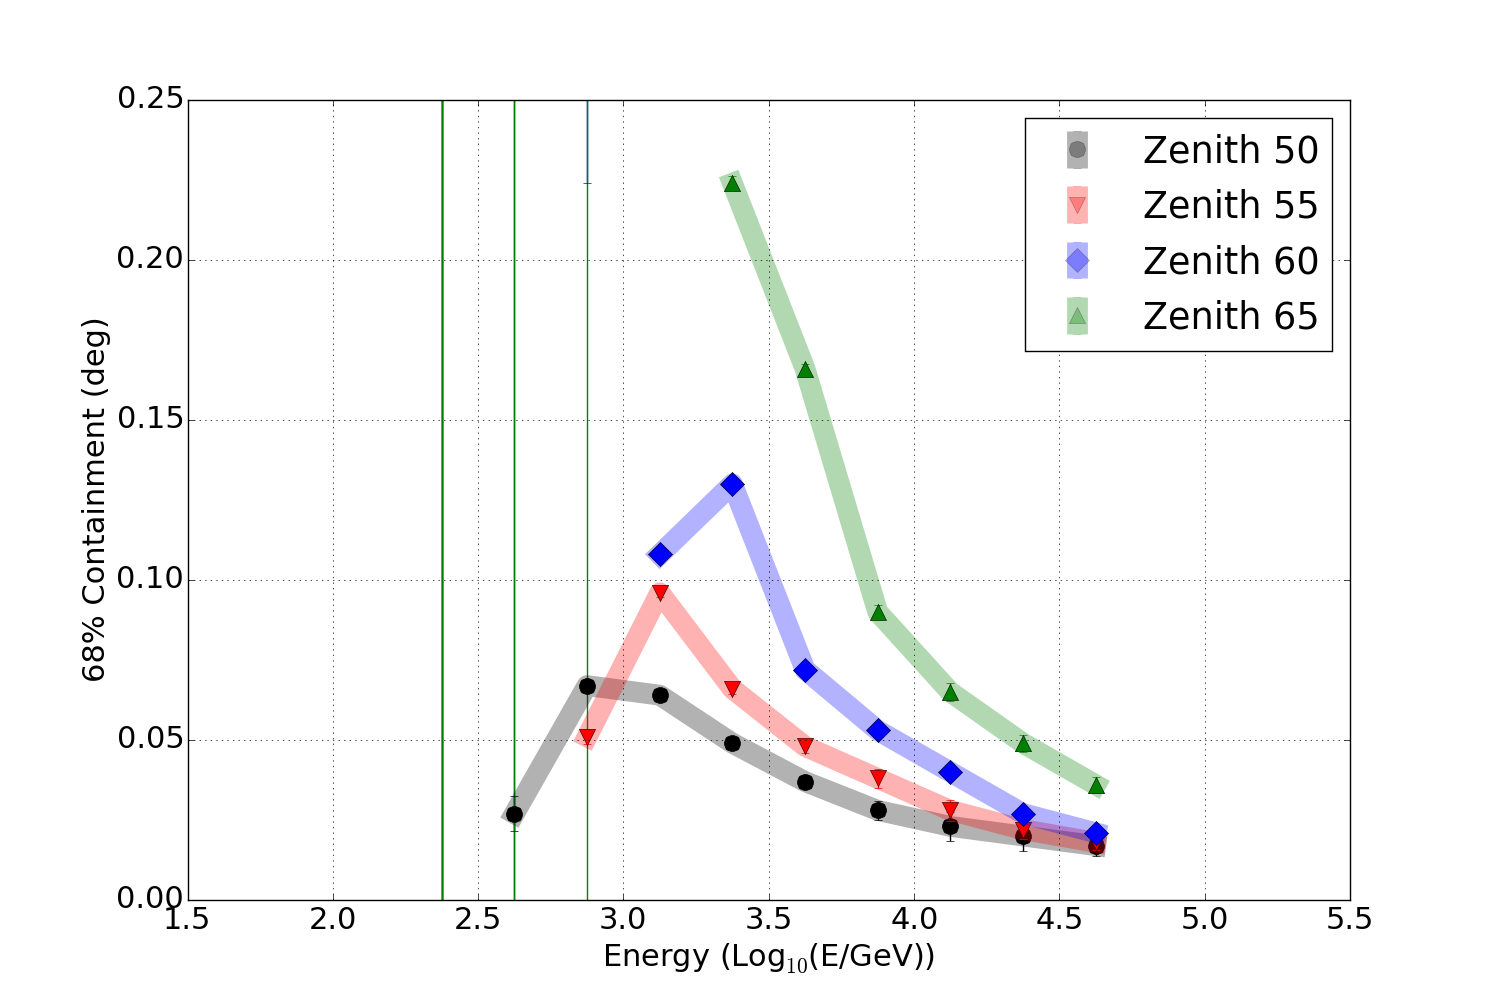
\includegraphics[width=.44\linewidth]{images/reg_energy_LZA}
    \label{fig:energy_reg_LZA}
  }
  \caption{Energy Dependence of Method0. Colored bands are intended to guide the eye and do not represent data points.}
  \label{fig:energy_reg}
\end{figure}

\begin{figure}[htbp]
  \centering
  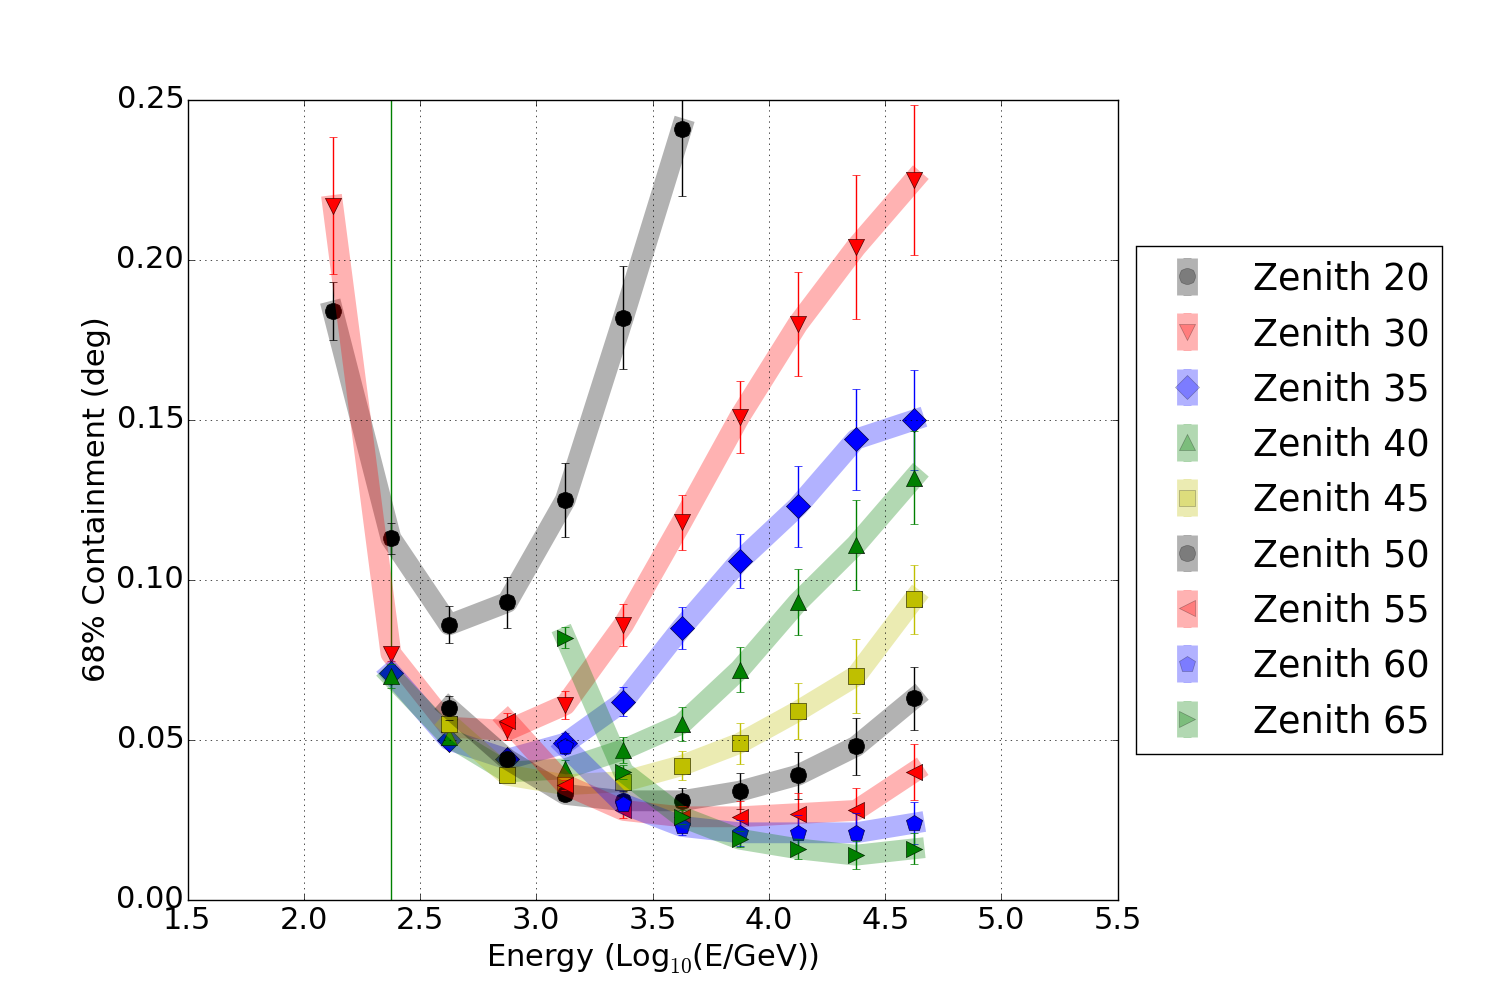
\includegraphics[width=.8\linewidth]{images/disp_standard_energy}
  \caption{Energy Dependence of the old Method5t. Colored bands are intended to guide the eye and do not represent data points.}
  \label{fig:energy_disp_standard}    
\end{figure}

\begin{figure}[htbp]
  \centering
  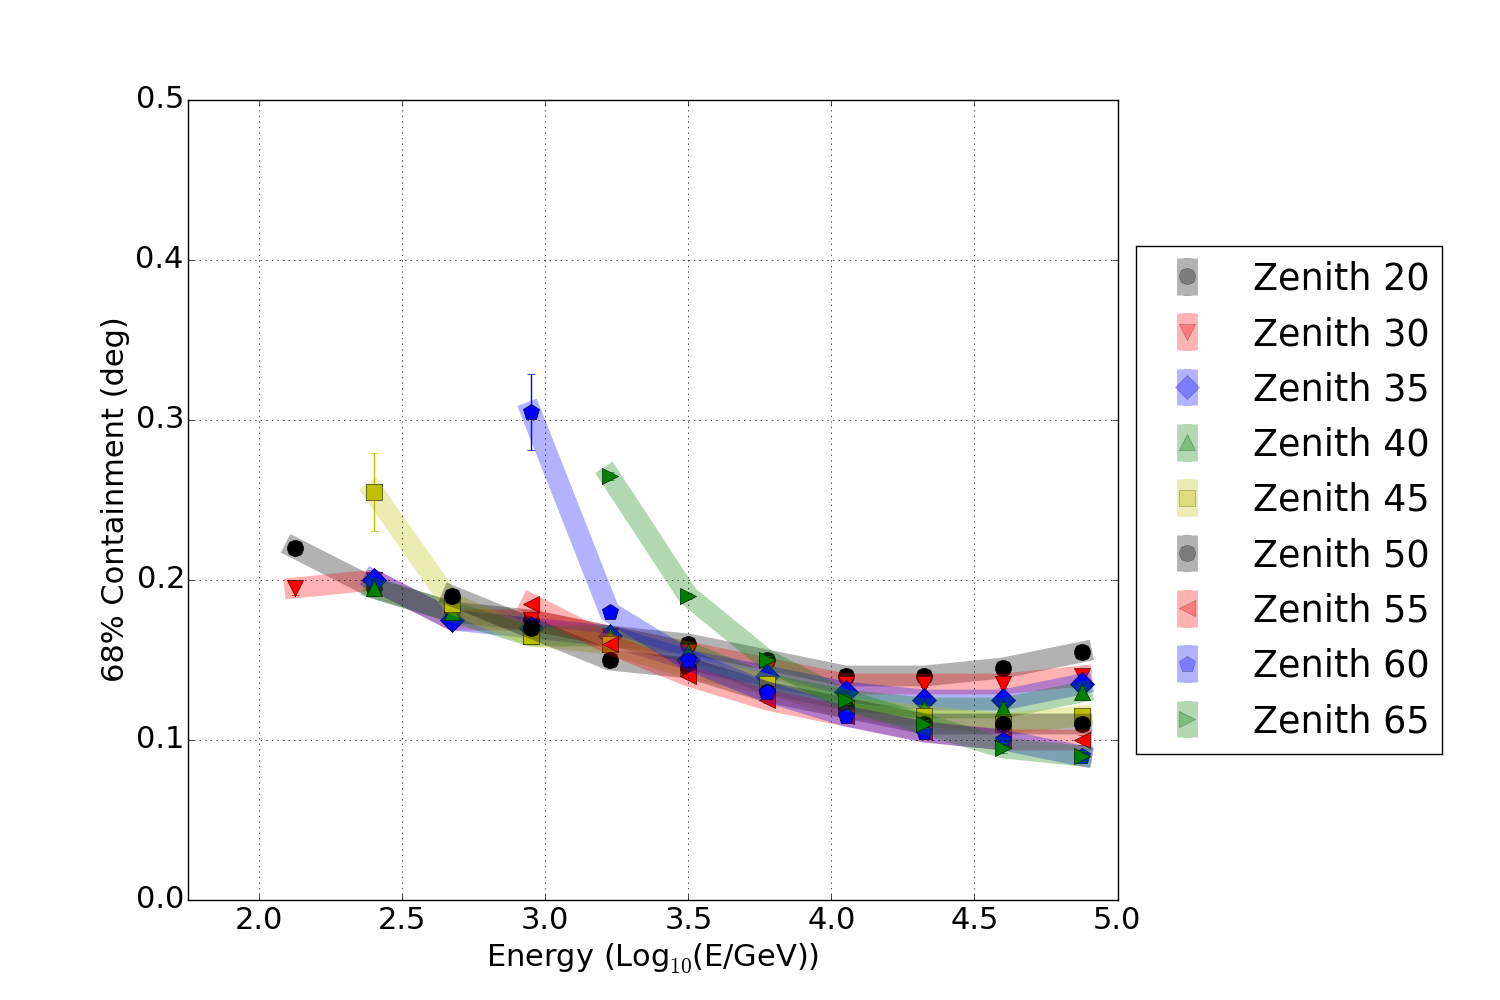
\includegraphics[width=.8\linewidth]{images/disp_450x4size_energy}
  \caption{Energy Dependence of the new Method5t. Colored bands intended to guide the eye and do not represent data points.}
  \label{fig:energy_disp_450}    
\end{figure}

The Method0 energy dependence (Fig. \ref{fig:energy_reg}) follows the same trend as in Fig. \ref{fig:disp_res} -- seeing the best resolution for all zeniths in the 3-30TeV range as well as a low energy improvement likely driven by high statistics. The energy dependence for the older \disp tables (Fig. \ref{fig:energy_disp_standard}) appears to have a minimum in \rse close to 1 TeV. These old \disp tables also see a degradation in resolution at the highest energies. The newer \disp tables (Fig. \ref{fig:energy_disp_450}) on the other hand appears to do {\bf better at higher energies for all zenith angles}. At energies above $\sim 1$ TeV and zenith angle greater than $30^\circ$, the \rse is at or better than $0.3^\circ$ (see Fig. \ref{fig:energy_new_contour}).

\begin{figure}[htbp]
  \centering
  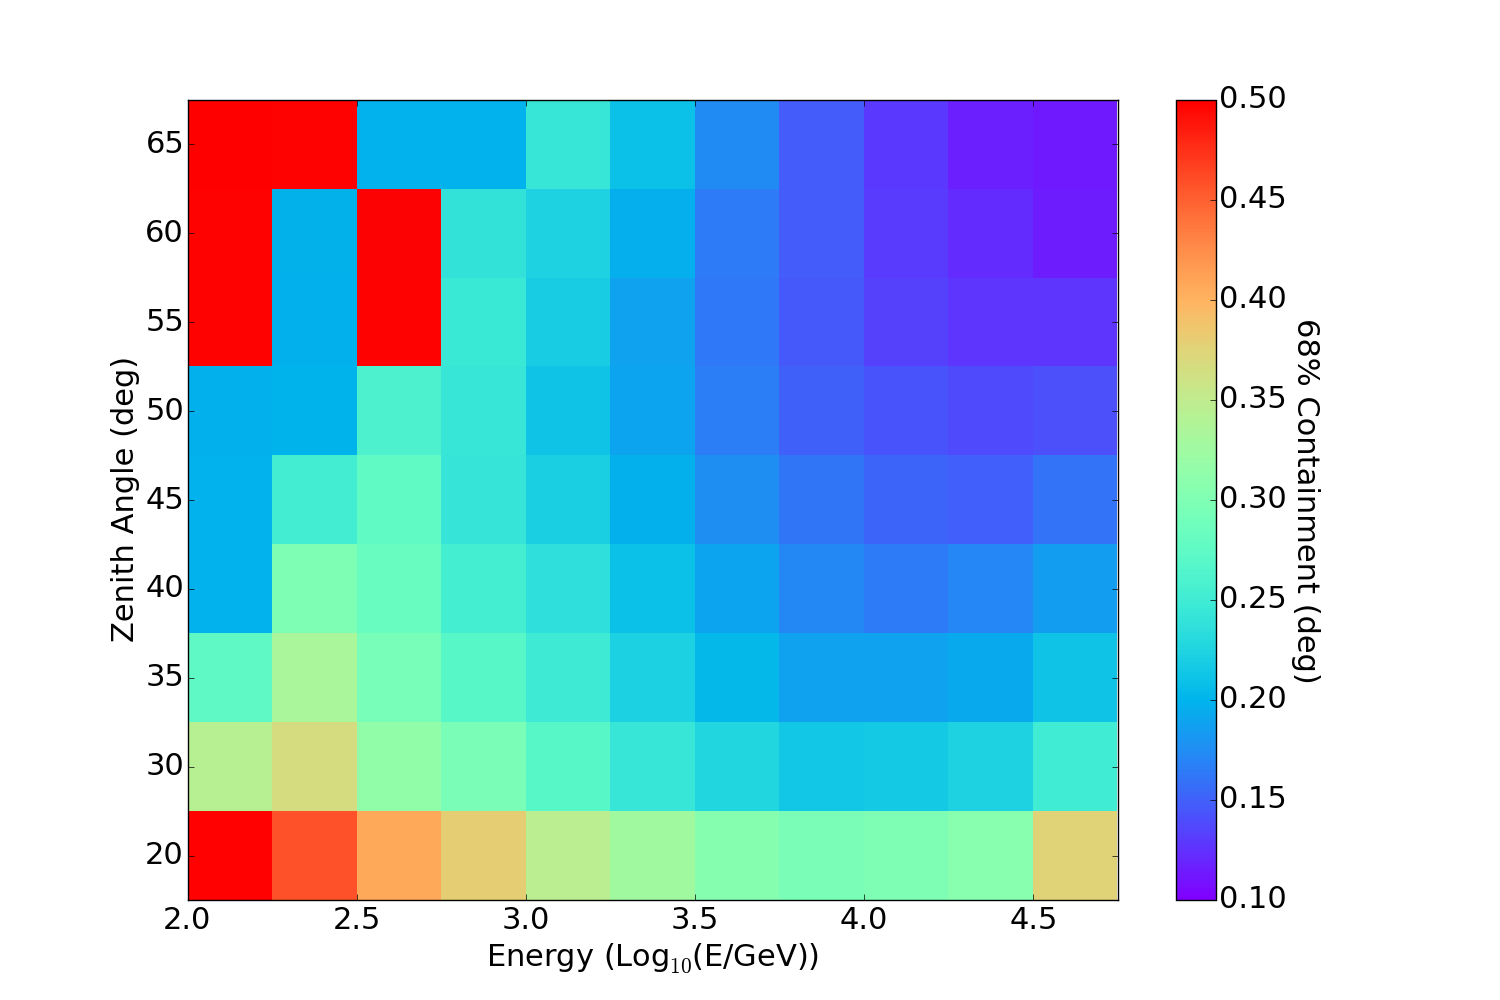
\includegraphics[width=.9\linewidth]{images/disp_450x4size_rse}
  \caption[Energy and zenith dependence of the new Method5t.]{Energy and zenith dependence of the new Method5t, with colors denoting the \rse and red denoting \rse$>=0.60^\circ$. The upper-left corner shows regions of loss in resolution in the large-zenith low-energy region, this is due to low statistics.}
  \label{fig:energy_new_contour}
\end{figure}

\begin{figure}[htbp]
  \centering
  \subfigure{
    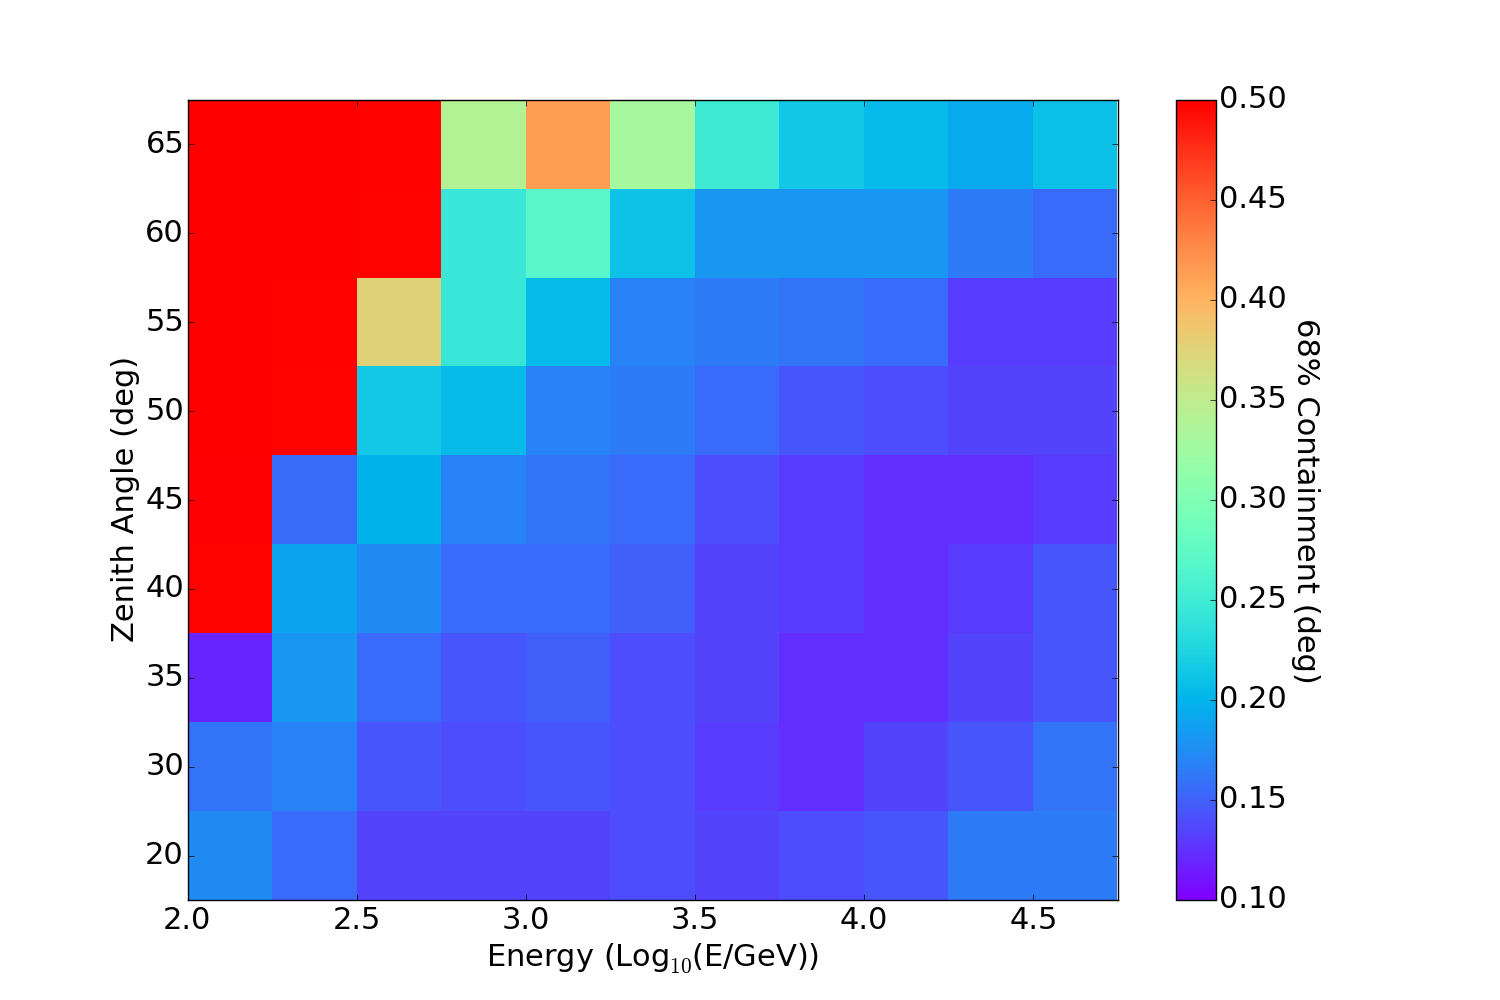
\includegraphics[width=0.47\linewidth]{images/reg_rse}
  }
  \subfigure{
    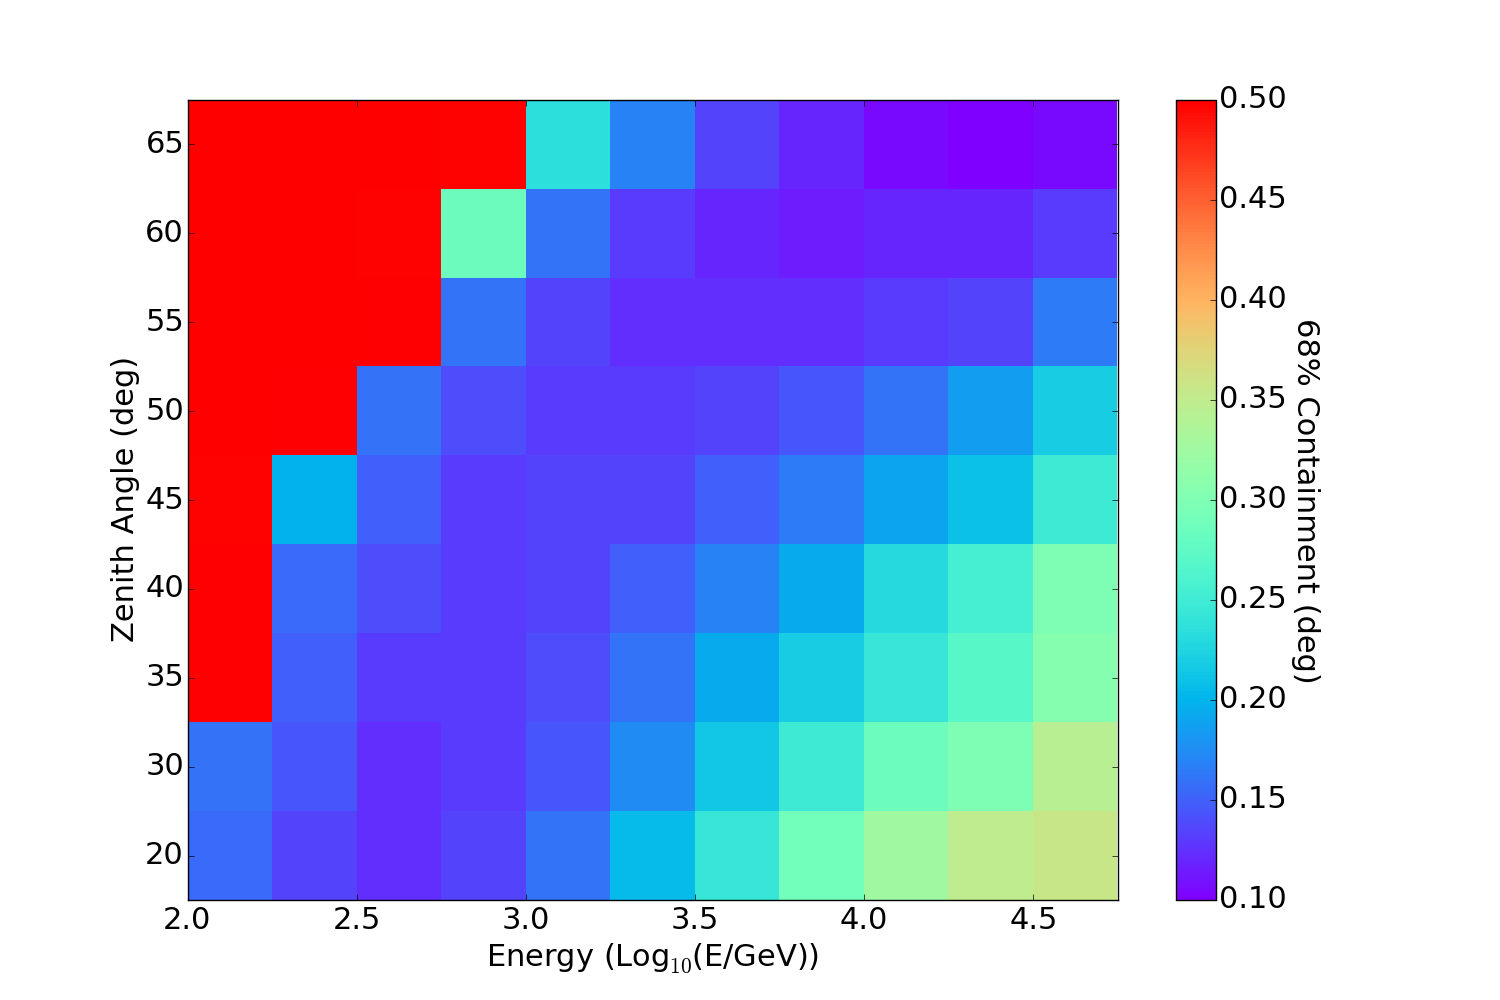
\includegraphics[width=0.47\linewidth]{images/disp_standard_rse}
  }
  \caption[Energy and zenith dependence of Method0 and the old Method5t]{Energy and zenith dependence of the geometric reconstruction (left) and the old Method5t (right), with colors denoting the \rse and red denoting \rse$>=0.60^\circ$.}
  \label{fig:energy_contour}
\end{figure}

\begin{figure}[htbp]
  \centering
  \subfigure{
    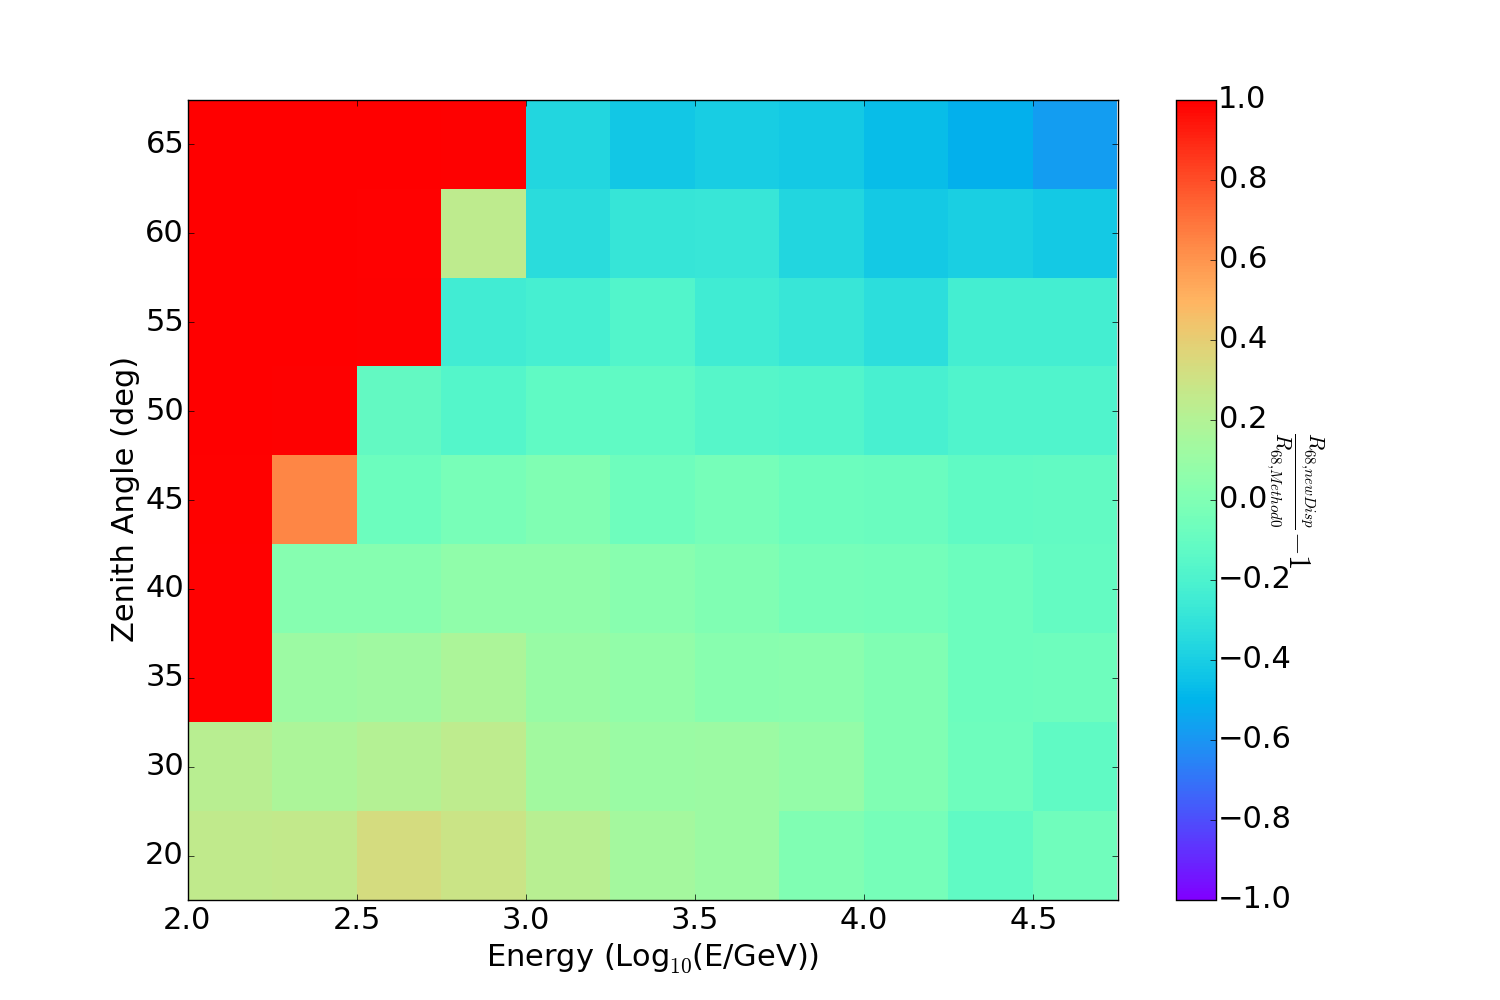
\includegraphics[width=0.47\linewidth]{images/rel_reg_sim}
  }
  \subfigure{
    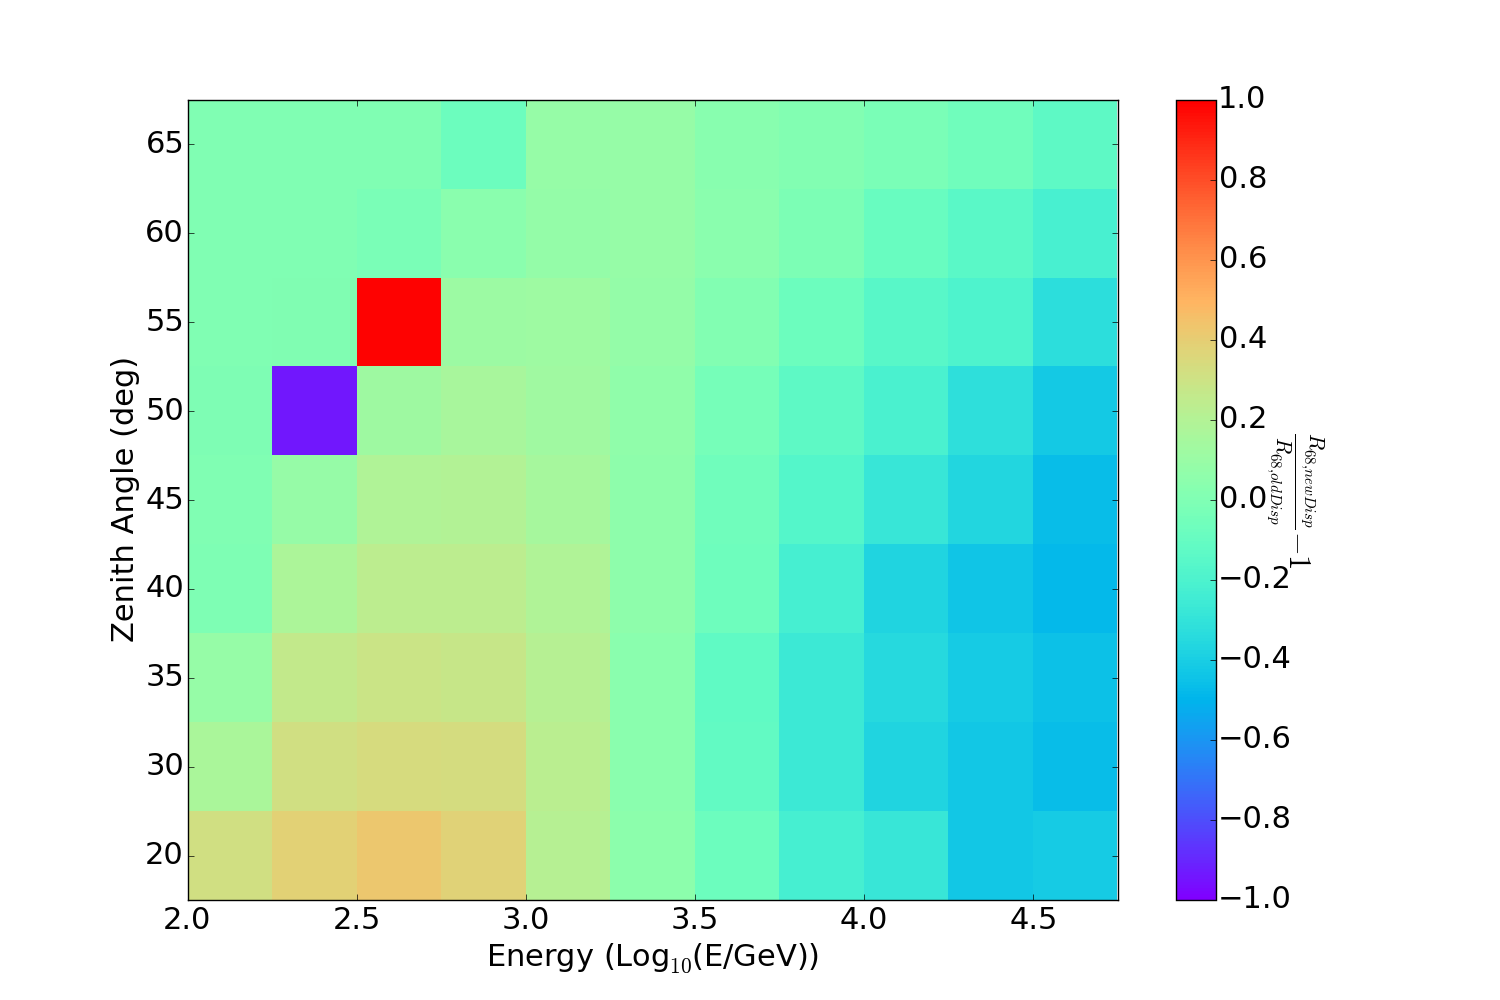
\includegraphics[width=0.47\linewidth]{images/rel_standard_sim}
  }
  \caption[Performance of the new \disp method compared to Method0 and the old \disp method]{Performance of the new \disp method compared to Method0 and the old \disp method, with colors denoting the \rse and red denoting $\frac{R_{68, \tx{new \disp}}}{R_{68, \tx{old \disp}}}-1>=1$ or  $\frac{R_{68, \tx{new \disp}}}{R_{68, \tx{reg}}}-1>=1$. The range of usefulness for Method5t (relative to Method0) now extends to $E>1$TeV and $\phi>=55^\circ$.}
  \label{fig:energy_rel}
\end{figure}

% Because the best resolution contours strongly constrain the parameter space to regions where statistics are low, constraints were used that were not simple rectangles. Instead an effective lower Reimann sum was used to construct an approximation that maximized the usable parameter space while imposing the most conservative constraints on parameter space between the simulated zenith values.
\section{\rse for Known Objects}
In order to test the validity of the results from the simulations, a known point-source with sufficient data collection at LZA and a hard spectrum (and therefore high statistics in the TeV range) was needed. Since our initial test was performed on the Crab Nebula and, in the VERITAS archival data it is the known object with the longest total exposure time at LZA, the Crab was used to generate some benchmarks. Additional objects considered for this were the Mrk421 and PKS1510-089.

\subsection{\rse for the Crab Nebula}

The Crab Nebula is expected to have a GeV-TeV extension of $\sim 0.03^\circ$ \cite{Fermi_LAT_Crab_extension}\cite{HESS_Crab_extension}. To observe this, a \rse of at least $0.03^\circ$ is required which, based on the simulations, we do not achieve. This however provides another metric by which to quantify our resolution, as well as to measure future gains in resolution.

% This is achieved at zenith angles of $45^\circ$ and greater and above $10^{4}$ GeV with the new \disp method. Due to small number statistics in the Crab data (as well as other observed data) in this region of parameter space, the criteria for this work were loosened to include zenith above $40^\circ$ and energies above $10^{3.5}$ GeV.
% Although this \rse is expected to be insufficient to \textit{measure} the GeV-TeV extension of the Crab due to low statistics, this can be used to demonstrate it \cite{Yeung:energy_extension}.

\begin{figure}[H]
  \begin{center}
    \subfigure[Angular resolution using Method5t.]{ 
      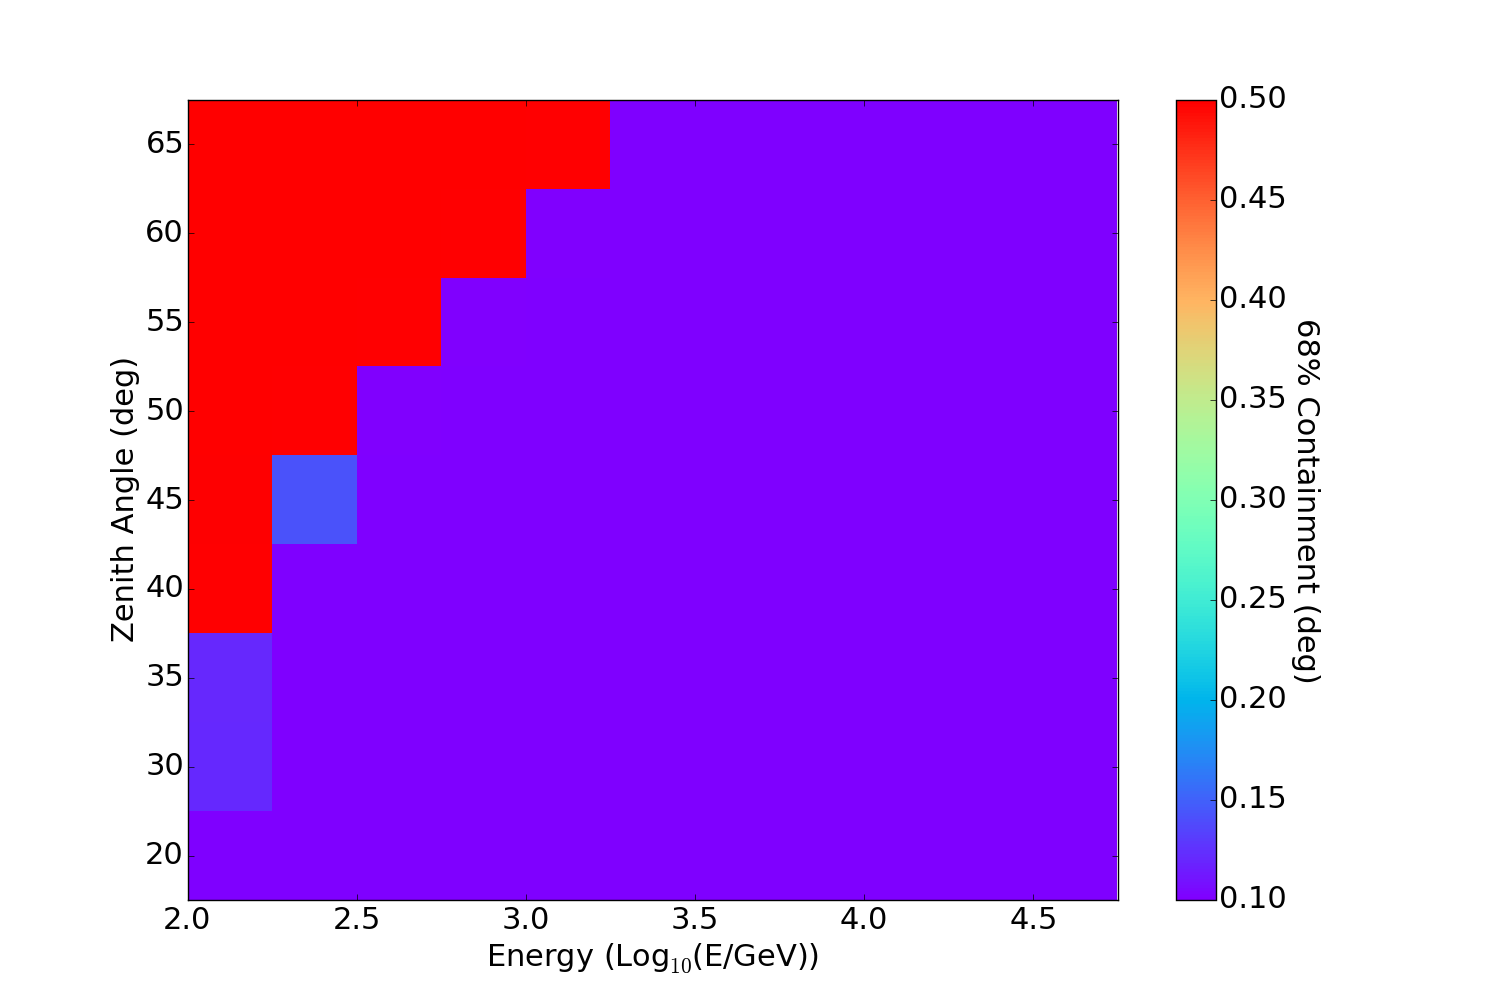
\includegraphics[width=0.47\linewidth]{crab_disp_rse.png}
      \label{fig:crab_disp_rse}
    }  
    \subfigure[Deviation from simulations.]{ 
      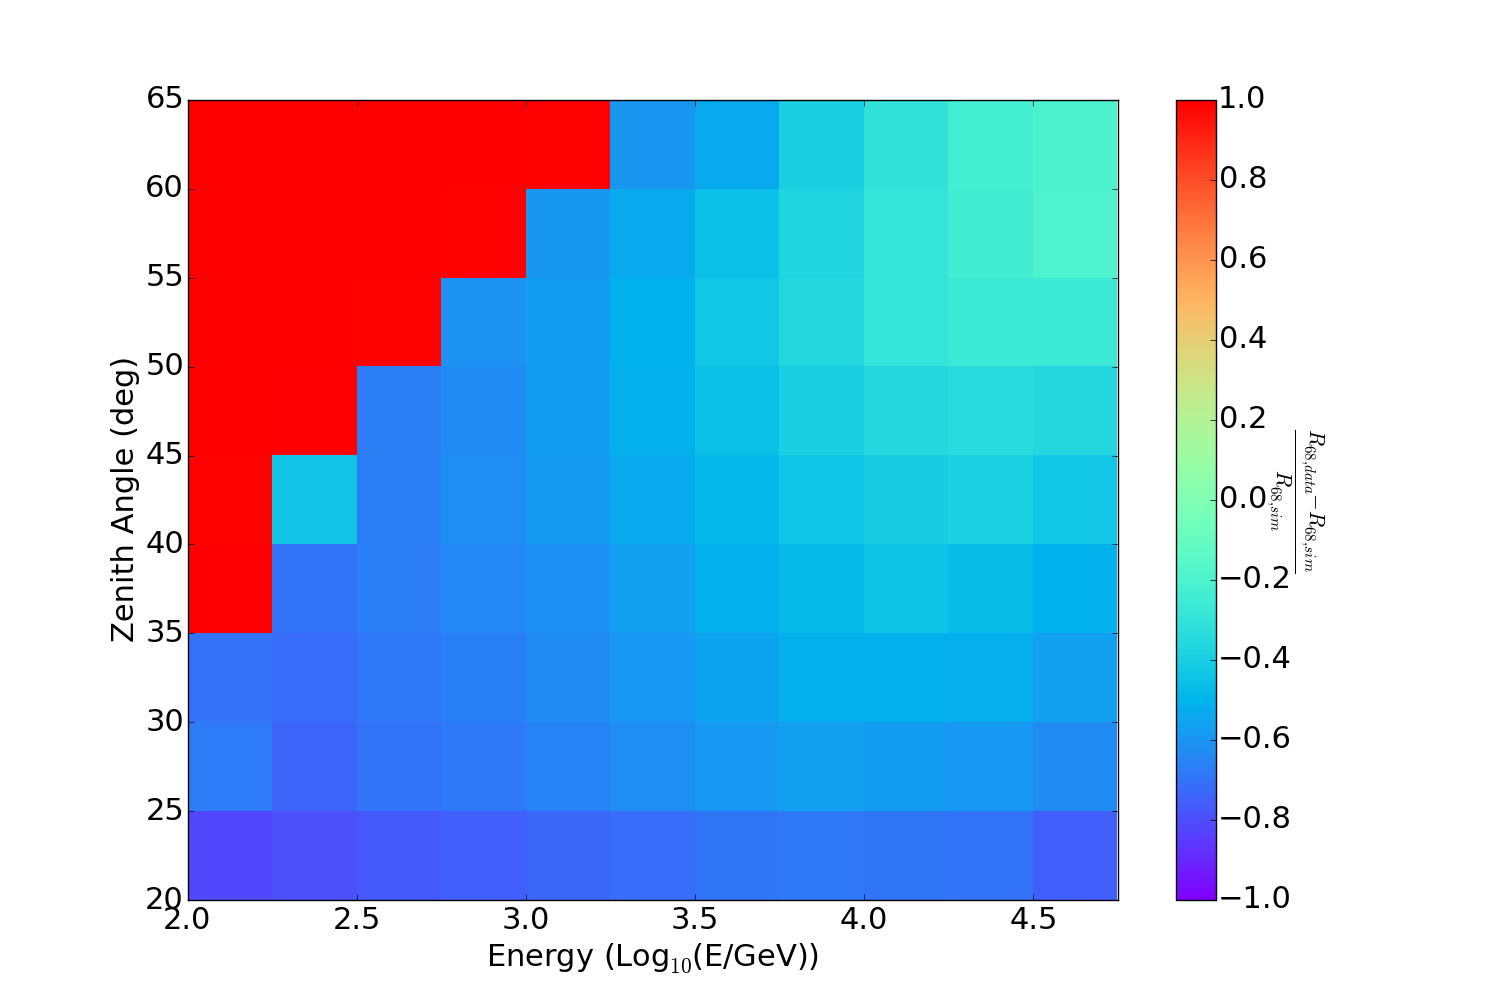
\includegraphics[width=0.47\linewidth]{crab_disp_sim.png}
      \label{fig:crab_disp_sim}
    }
    \subfigure[Number of events ($\log(N_{on}-\alpha N_{off})$).]{ 
      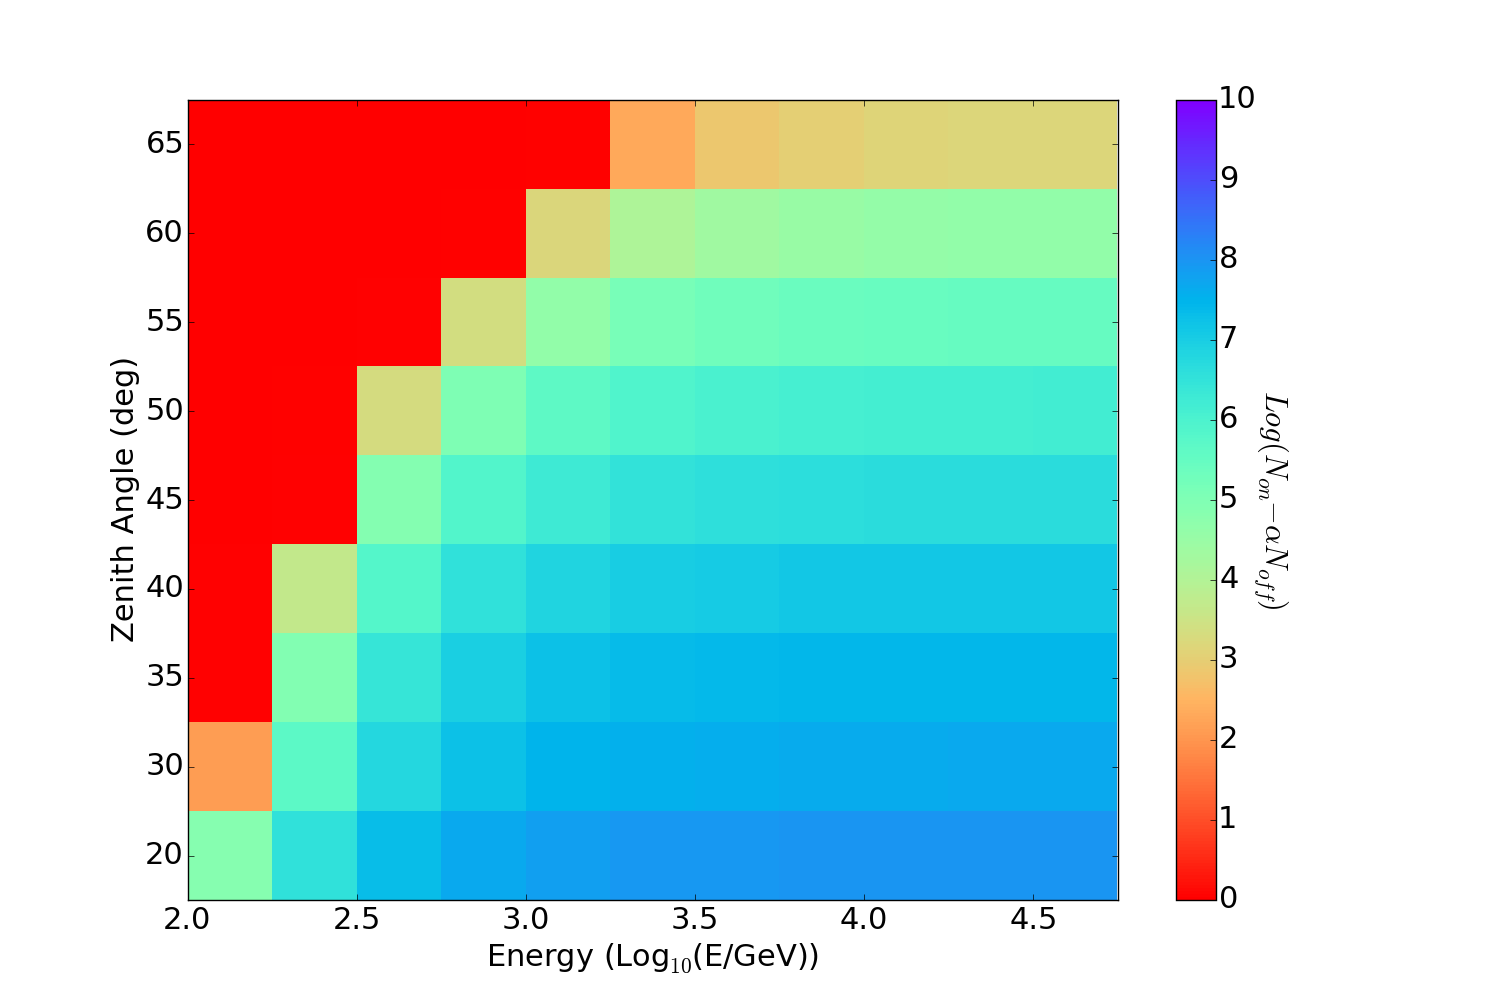
\includegraphics[width=0.47\linewidth]{crab_disp_Log_nevent.png}
      \label{fig:crab_disp_nevent}
    }  
    \subfigure[Li \& Ma significance.]{ 
      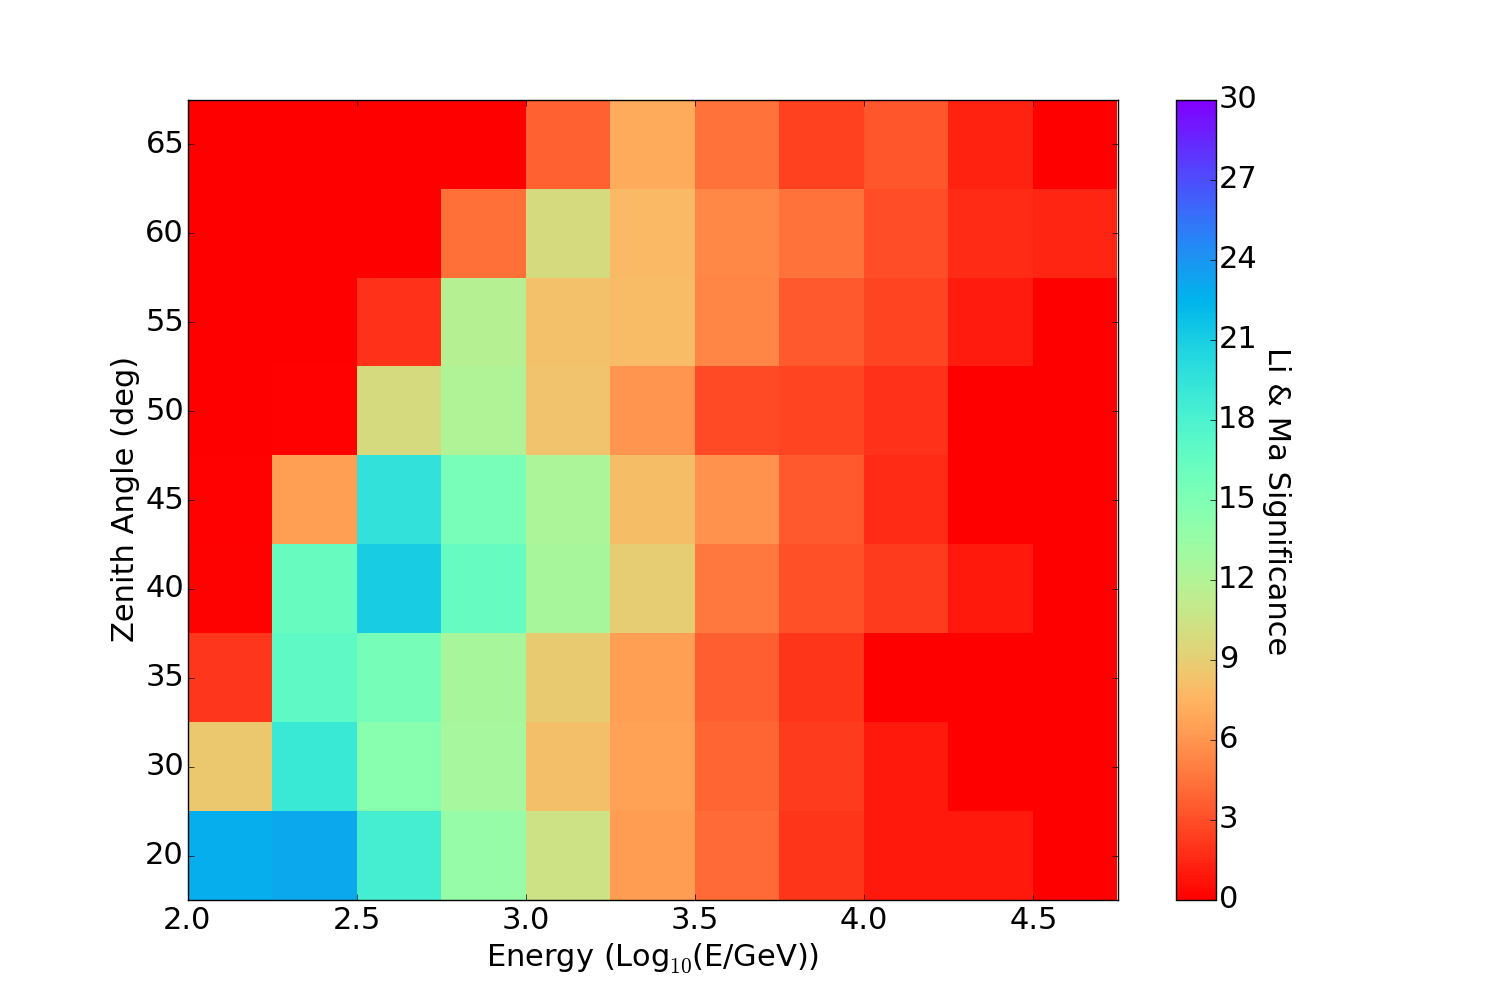
\includegraphics[width=0.47\linewidth]{crab_disp_LiMa.png}
      \label{fig:crab_disp_li_ma}
    }
  \end{center}
  \caption[Crab (horizon-to-horizon runs) direction reconstruction using Method5t.]{Reconstruction of the direction of the Crab Nebula horizon-to-horizon runs using the new \disp tables. In each case red denotes regions of no statistics.}
  \label{fig:crab_disp}
\end{figure}

\begin{figure}[H]
  \begin{center}
    \subfigure[Angular resolution using Method5t.]{ 
      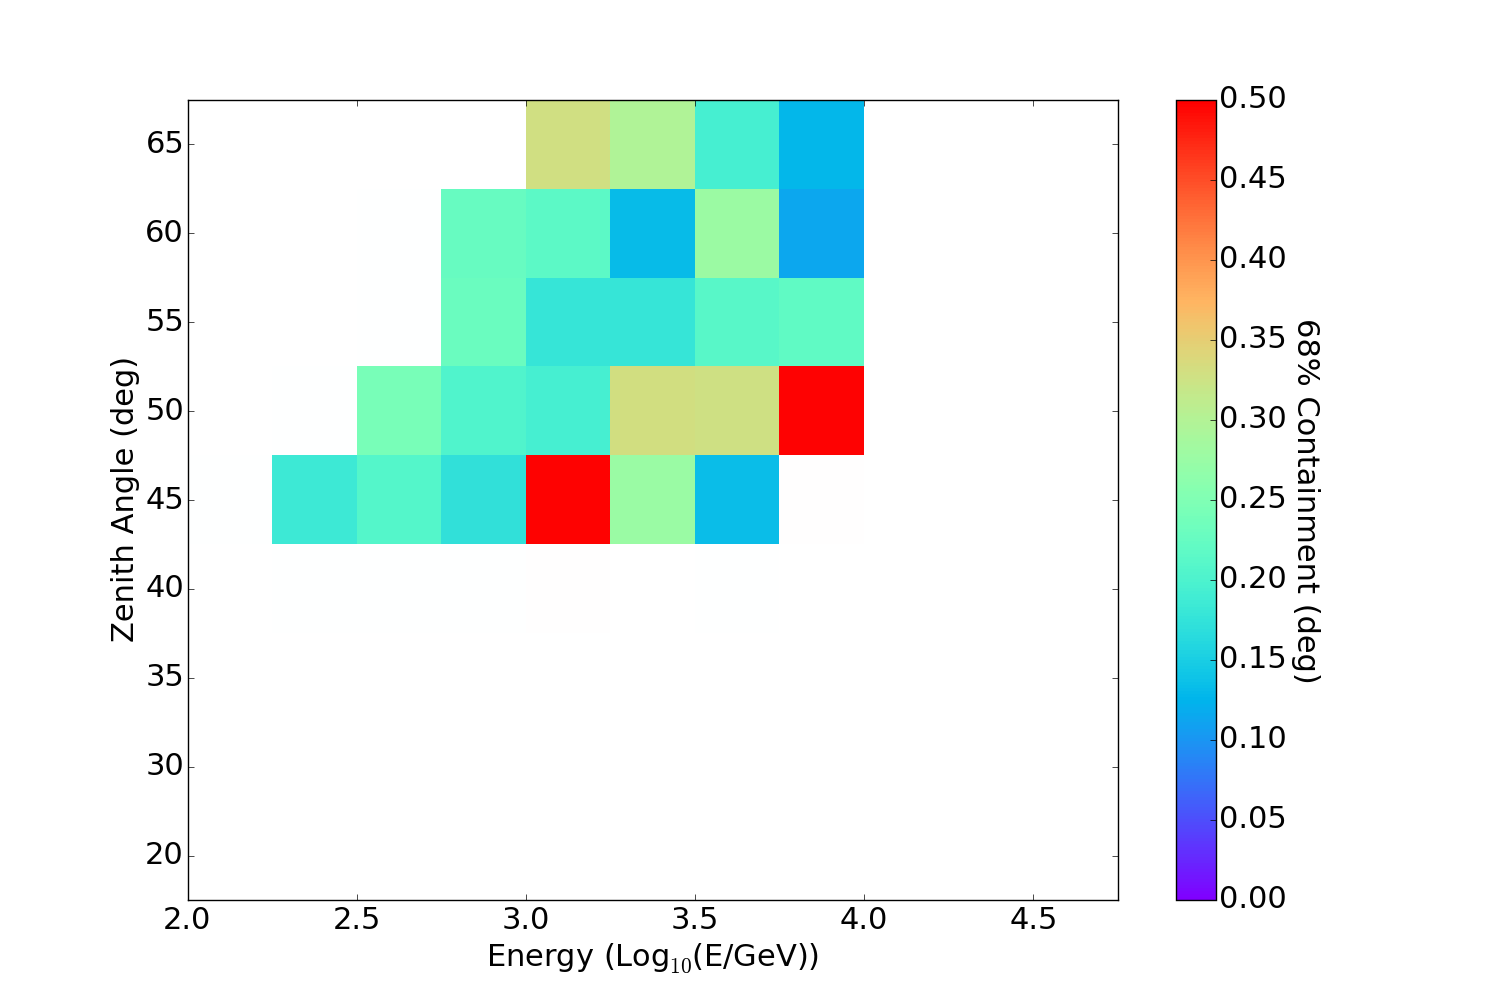
\includegraphics[width=0.47\linewidth]{crab_all_disp_rse.png}
      \label{fig:crab_all_disp_rse}
    }  
    \subfigure[Deviation from simulations.]{ 
      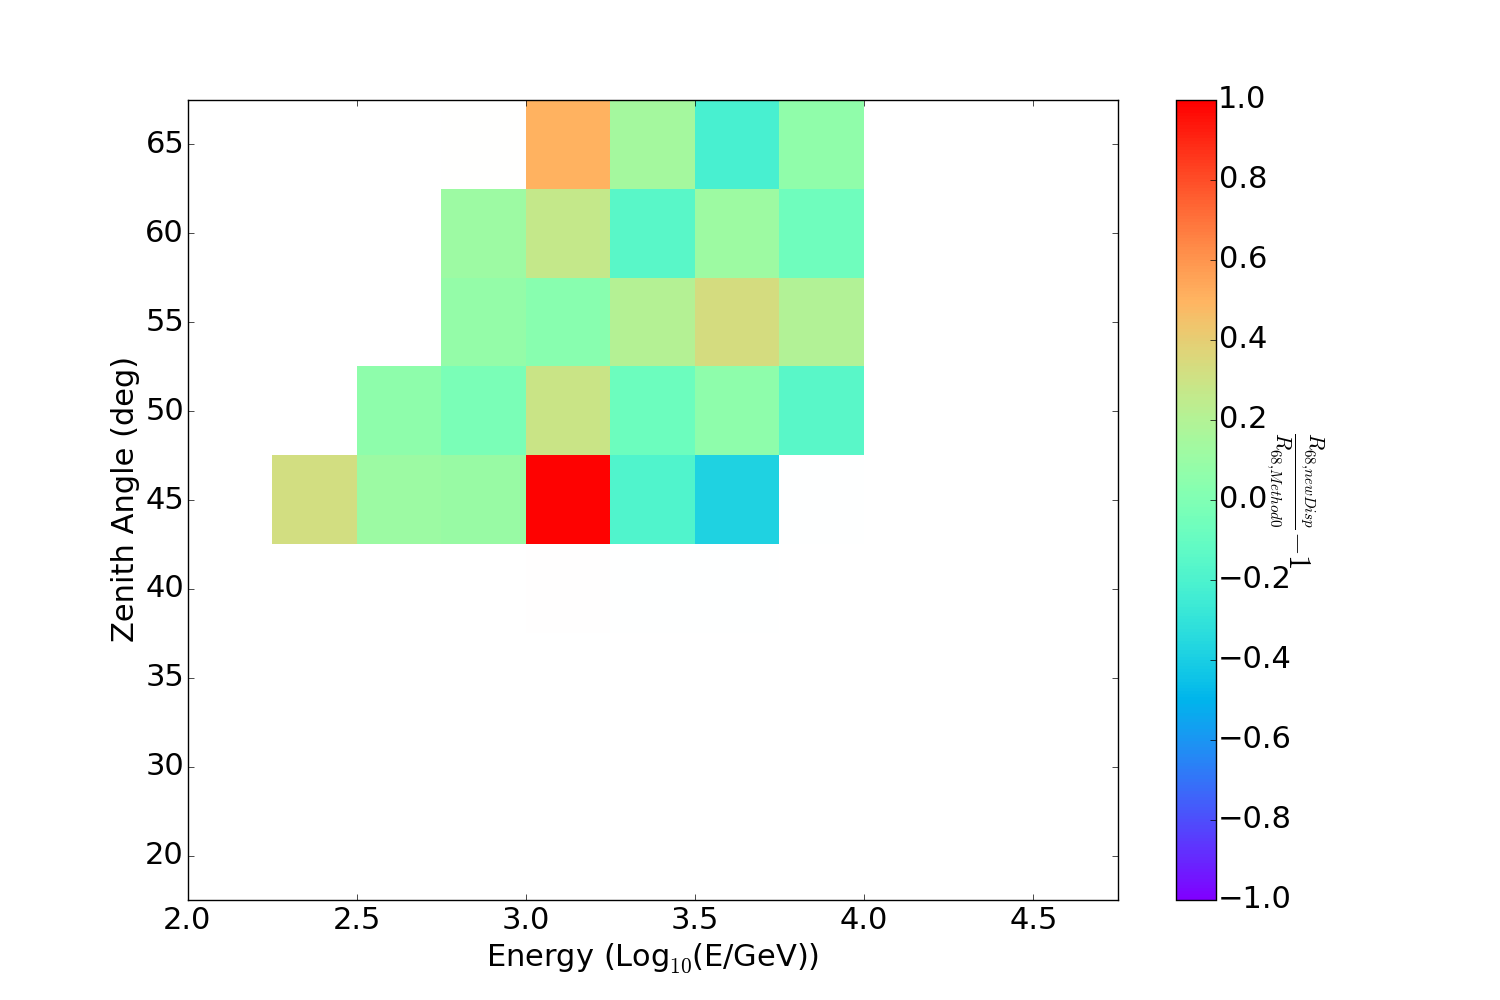
\includegraphics[width=0.47\linewidth]{crab_all_disp_sim.png}
      \label{fig:crab_all_disp_sim}
    }
    \subfigure[Number of events ($\log(N_{on}-\alpha N_{off})$).]{ 
      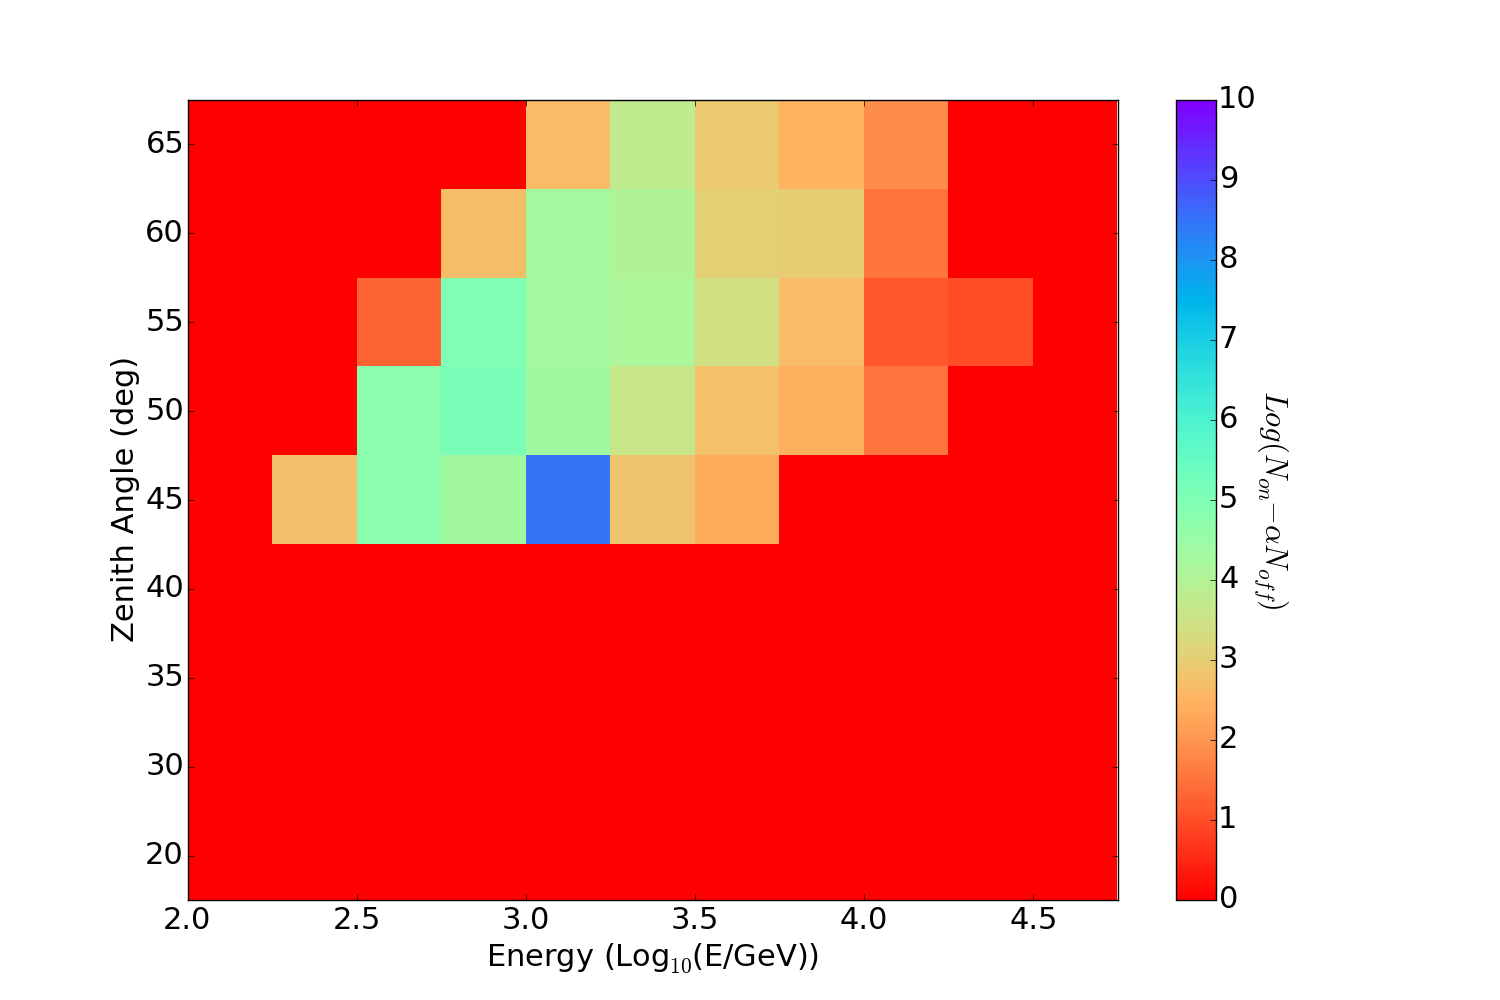
\includegraphics[width=0.47\linewidth]{crab_all_disp_Log_nevent.png}
      \label{fig:crab_all_disp_nevent}
    }  
    \subfigure[Li \& Ma significance.]{ 
      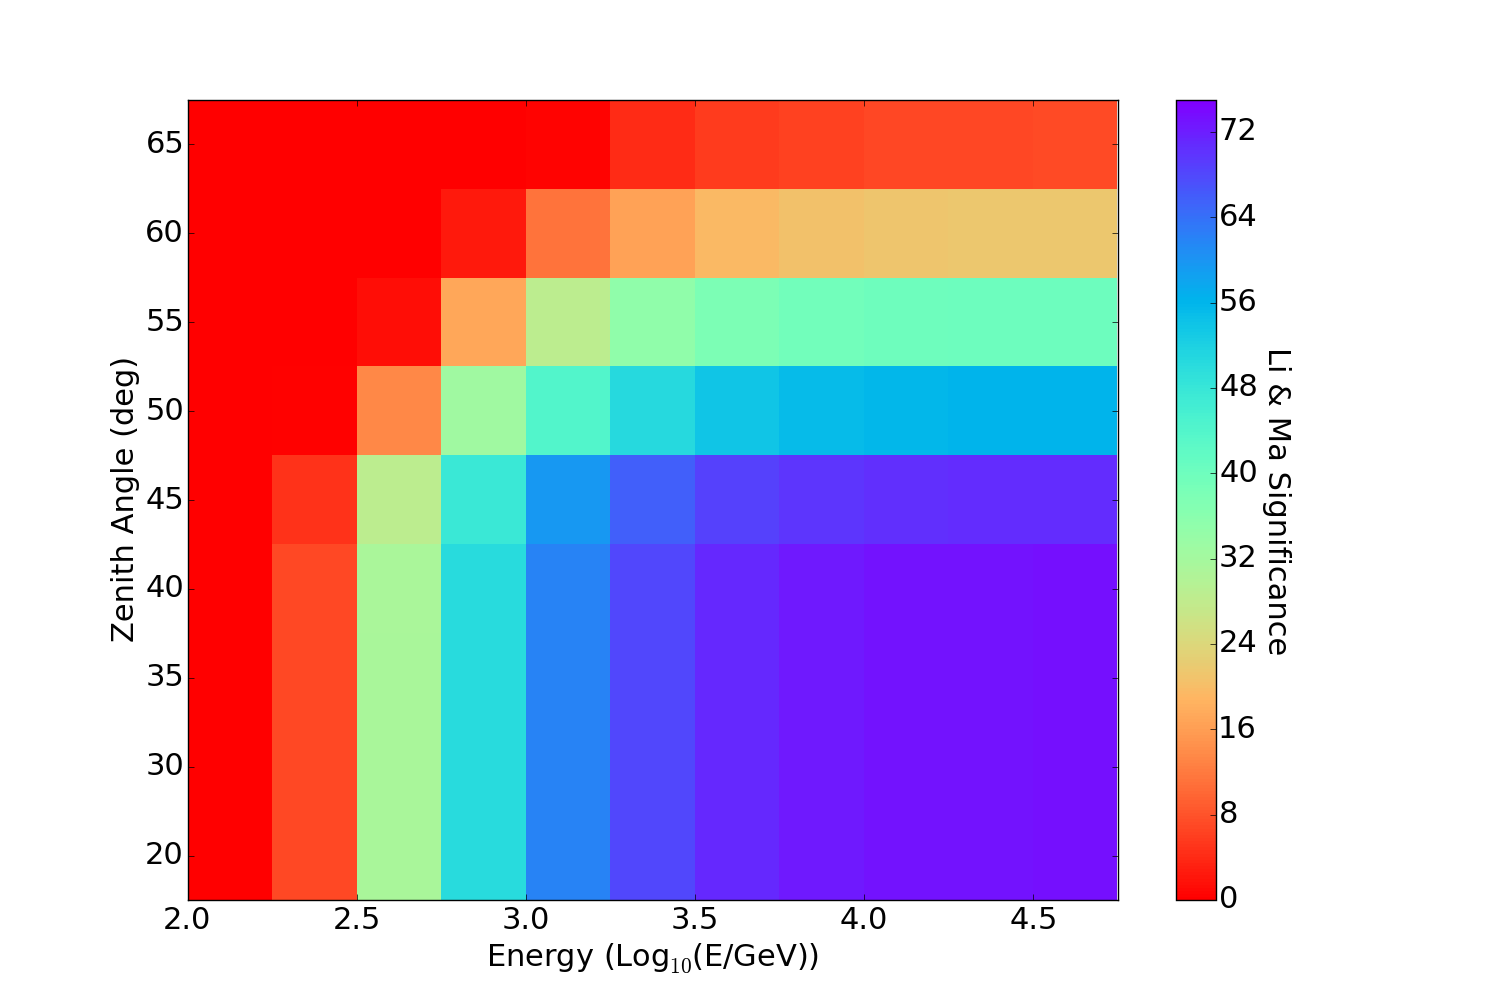
\includegraphics[width=0.47\linewidth]{crab_all_disp_LiMa.png}
      \label{fig:crab_all_disp_li_ma}
    }
  \end{center}
  \caption[Crab (LZA runs) direction reconstruction using Method5t.]{Reconstruction of the direction of the Crab Nebula LZA runs using the new \disp tables. In each case red denotes regions of no statistics.}
  \label{fig:crab_all_disp}
\end{figure}

The numbers for the Crab in Fig. \ref{fig:crab_disp} suggest that we can detect the extension of the Crab.

\subsection{\rse for Mrk421}
Mrk421 is an extra-galactic source ($z=0.031$) with a hard spectrum (spectral index $\Gamma=2.2$), but less than 5 hours of observation in the zenith range of interest ($\phi>40$). Even with a short total duration of observation, because Mrk421 is a high-flux object, it is still observable to high significance.

The result of this analysis was that the smallest values of \rse for Mrk421 ($\sim 0.08^\circ$) is found in a region of parameter space where the Li \& Ma significance is negligible.

\begin{figure}[H]
  \begin{center}
    \subfigure[Angular resolution using Method5t.]{ 
      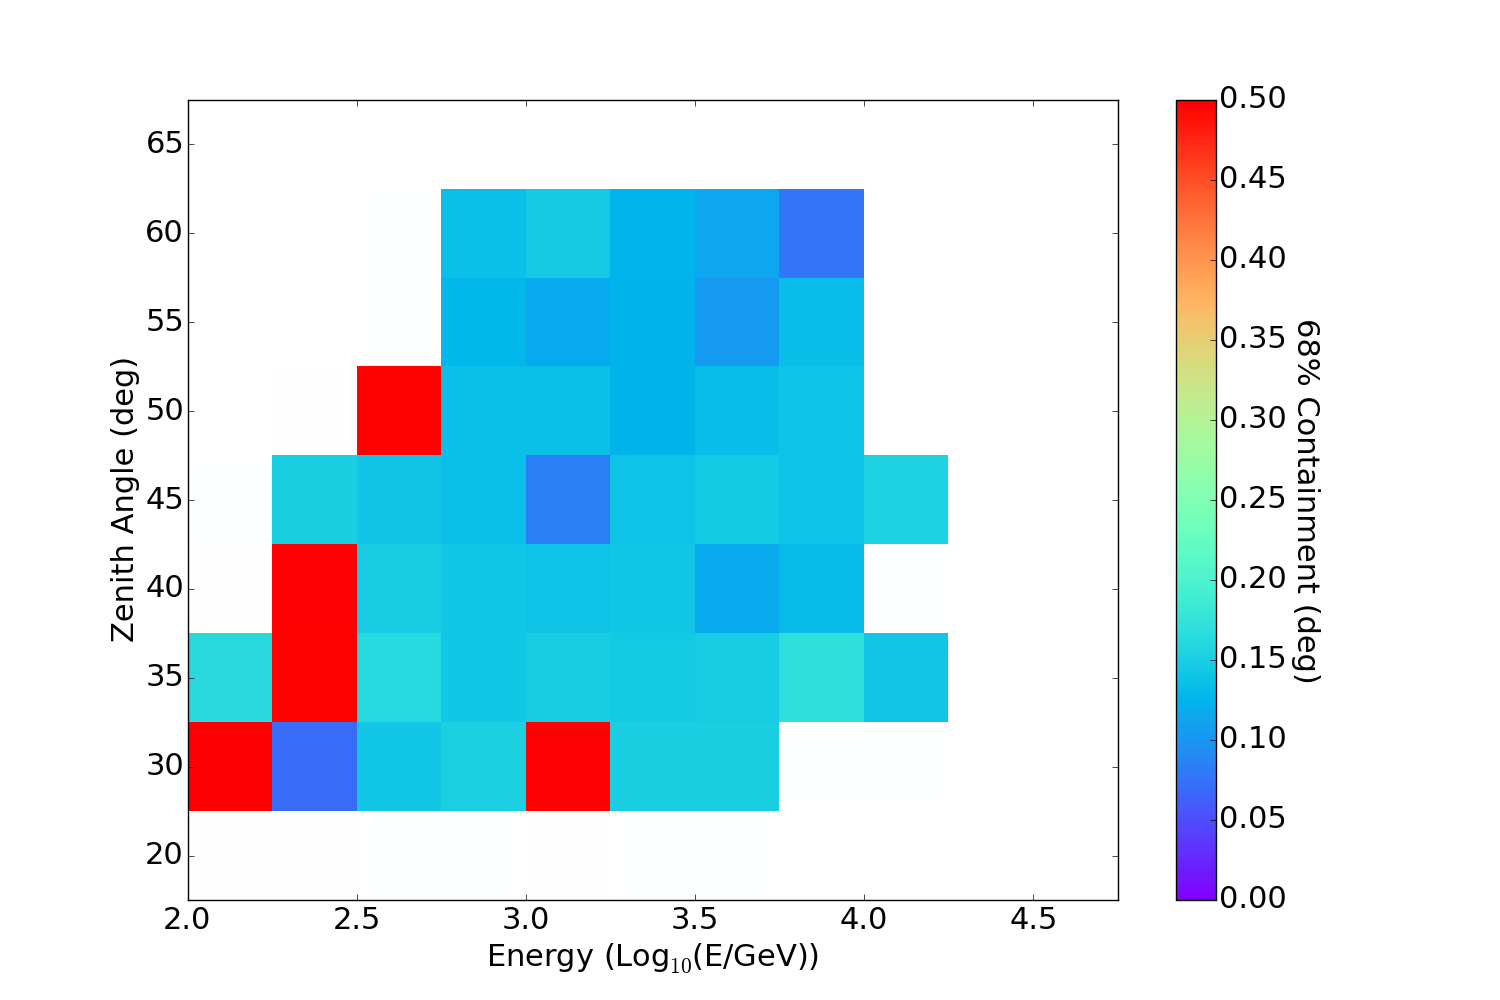
\includegraphics[width=0.47\linewidth]{Mrk421_rse.png}
      \label{fig:mrk_rse}
    }  
    \subfigure[Deviation from simulations.]{ 
      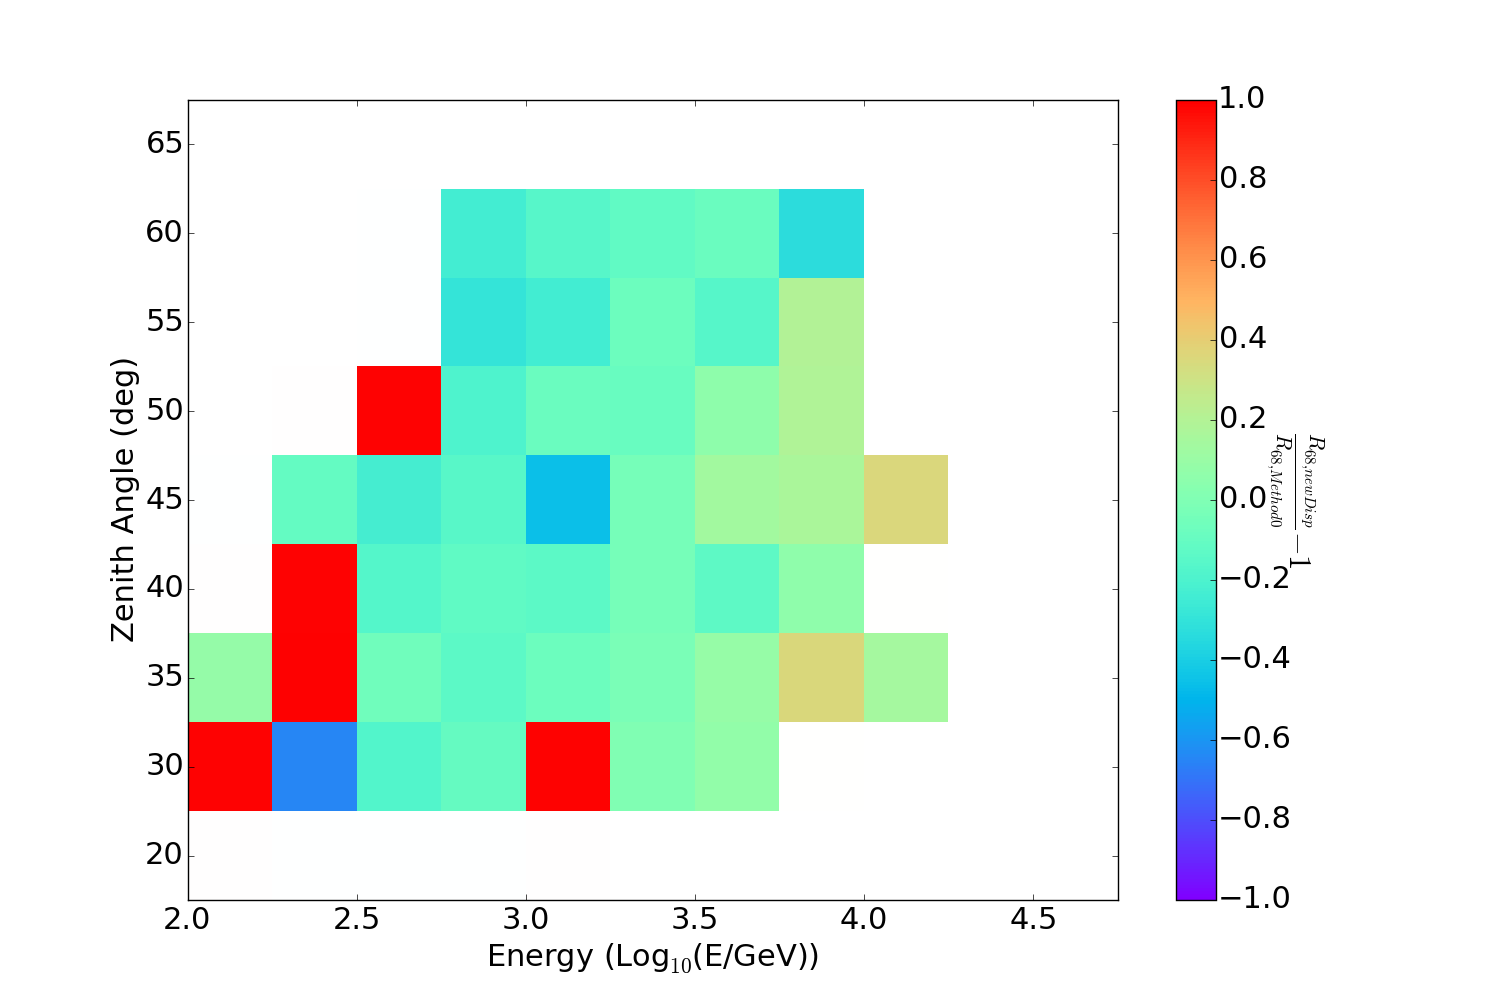
\includegraphics[width=0.47\linewidth]{Mrk421_sim.png}
      \label{fig:mrk_sim}
    }
    \subfigure[Number of events ($\log(N_{on}-\alpha N_{off})$).]{ 
      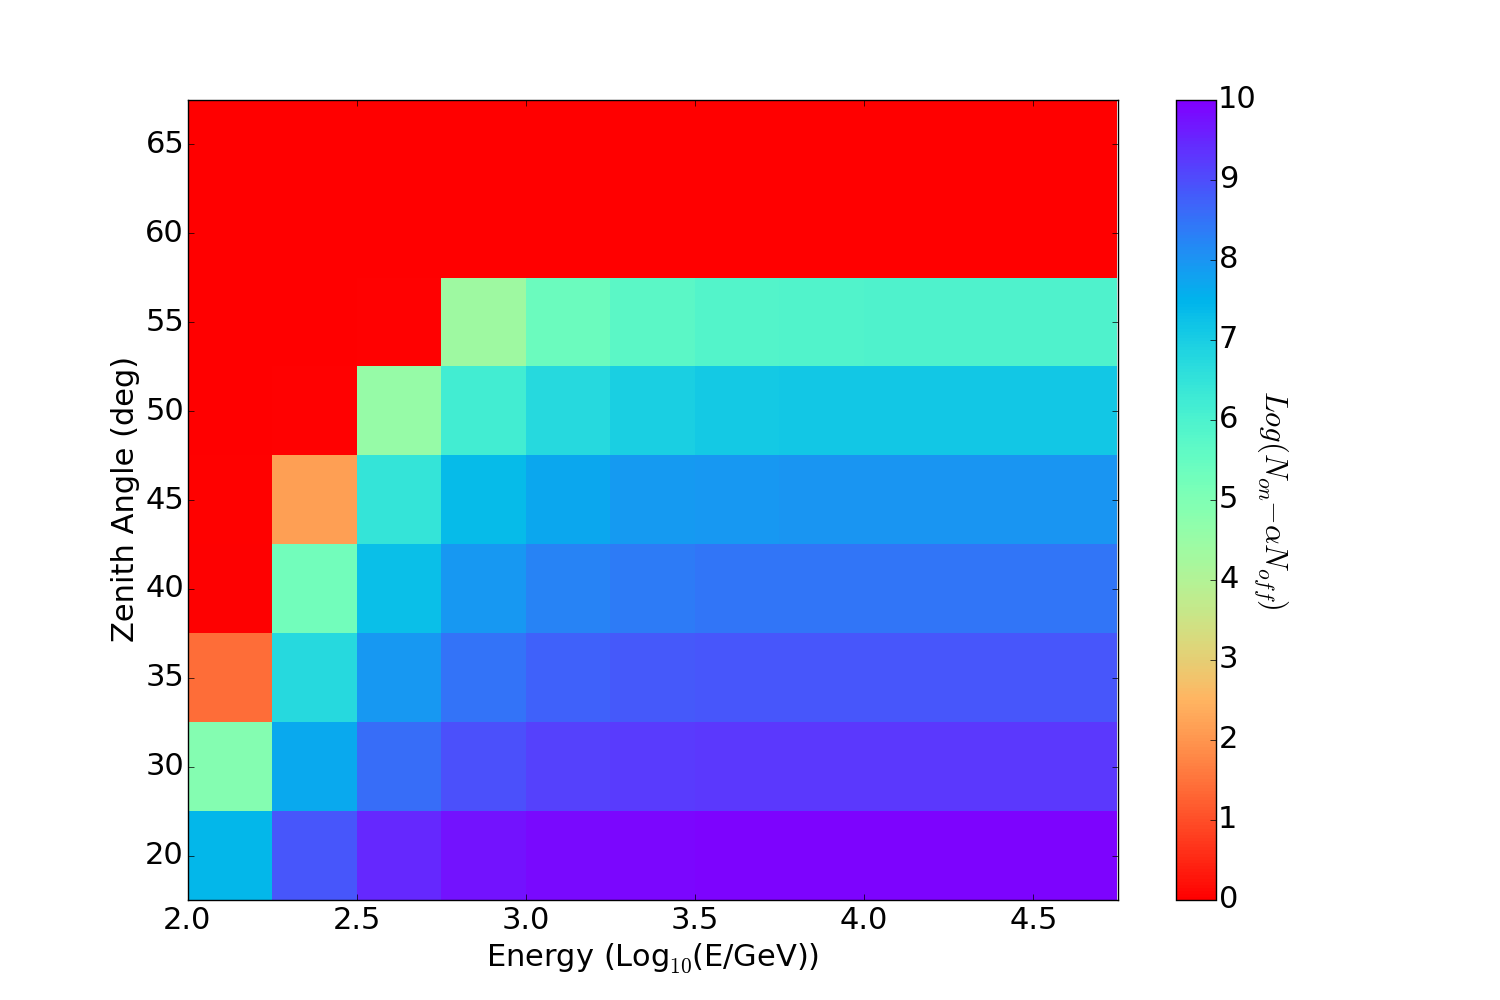
\includegraphics[width=0.47\linewidth]{Mrk421_Log_nevent.png}
      \label{fig:mrk_nevent}
    }  
    \subfigure[Li \& Ma significance.]{ 
      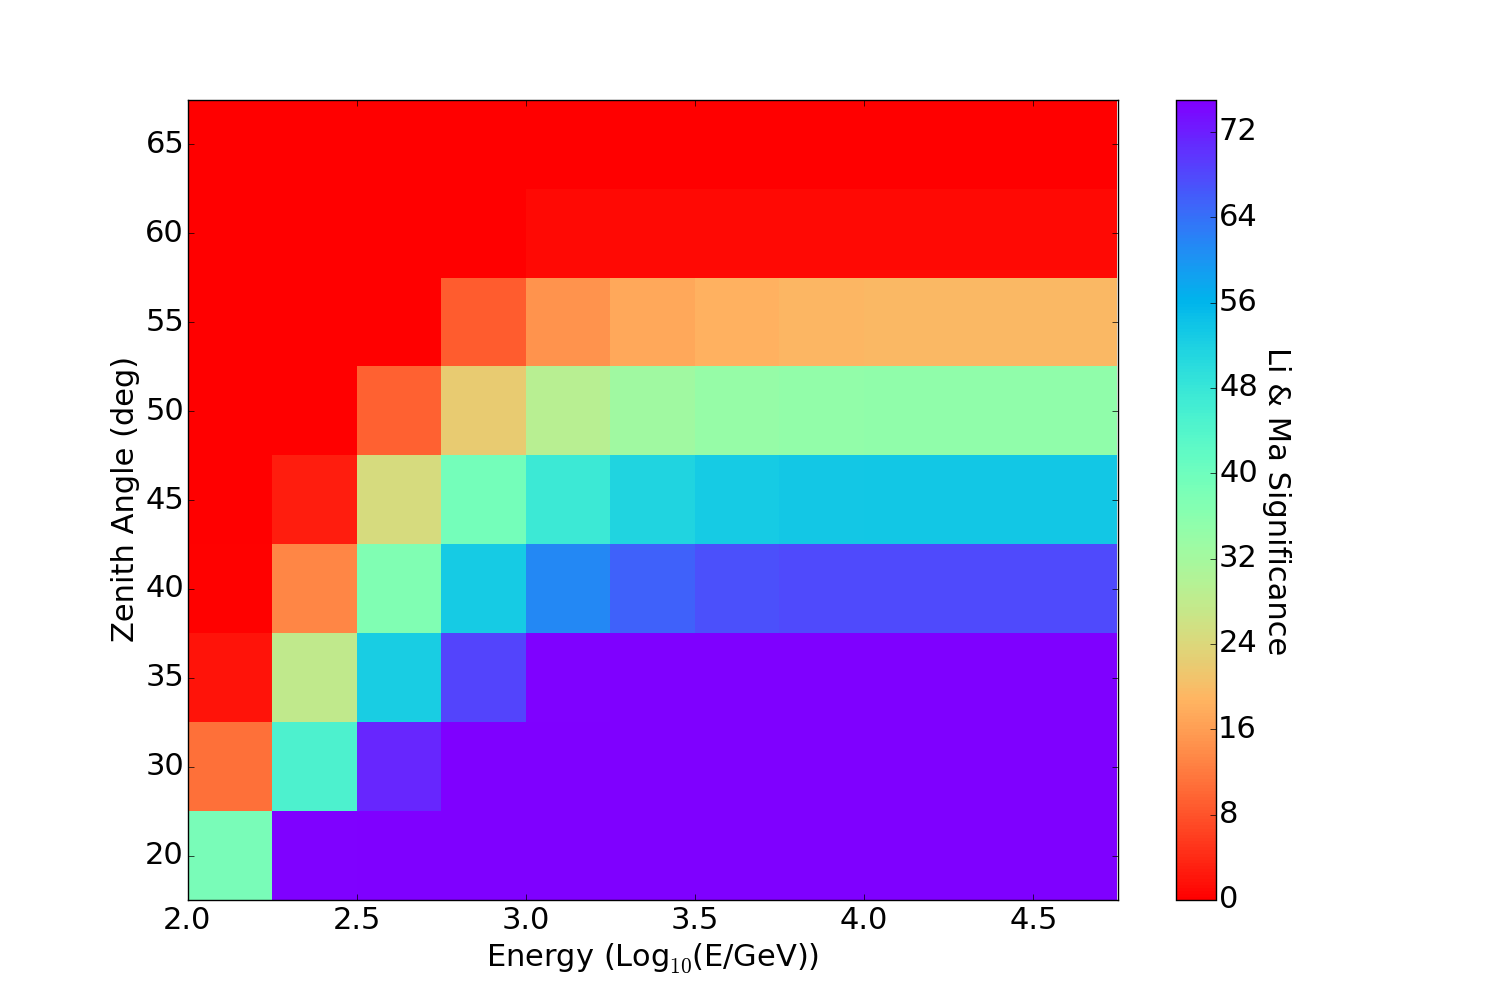
\includegraphics[width=0.47\linewidth]{Mrk421_LiMa.png}
      \label{fig:mrk_li_ma}
    }
  \end{center}
  \caption[Mrk421 direction reconstruction using Method5t.]{Reconstruction of the direction of Mrk421 using the new \disp tables. In each case red denotes regions of no statistics.}
  \label{fig:mrk_disp}
\end{figure}

\subsection{\rse for PKS1510-089}
PKS1510-089 is an extra-galactic source ($z=0.361$) with a softer spectrum (spectral index $\Gamma=3.26$), but 17 hours of observation in the zenith range of interest ($\phi>40$). Analysis of the data reveals that none of this falls in the region of best performance ($\phi>45$ and $E>10$TeV)

% \begin{table}[htbp]
%   \begin{center}
%     \begin{tabularx}{\textwidth}{ X | X | X | X | X }
%       \hline
%       \textbf{Min. Zenith (deg)} & \textbf{Min. Energy (TeV)} & \textbf{Min. Energy (Log$_{10}$($\frac{E}{GeV}$))} & \textbf{\rse (deg)} & \textbf{N$_{\rm{on}}$}\\
%       \hline\hline
%       45 & 10.0 & 4.0 & N/A & 0\\
%       40 & 3.16 & 3.5 & $0.7 \pm 2.0$ & 24\\
%       40 & 1.0 & 3.0 & $0.09 \pm 0.02$ & 128\\
%     \end{tabularx}
%     \caption[\rse for PKS1510-089.]{\rse for PKS1510-089 from a live time of 17.1 hours.}
%   \end{center}
% \end{table}

\begin{figure}[H]
  \begin{center}
    \subfigure[Angular resolution using Method5t.]{ 
      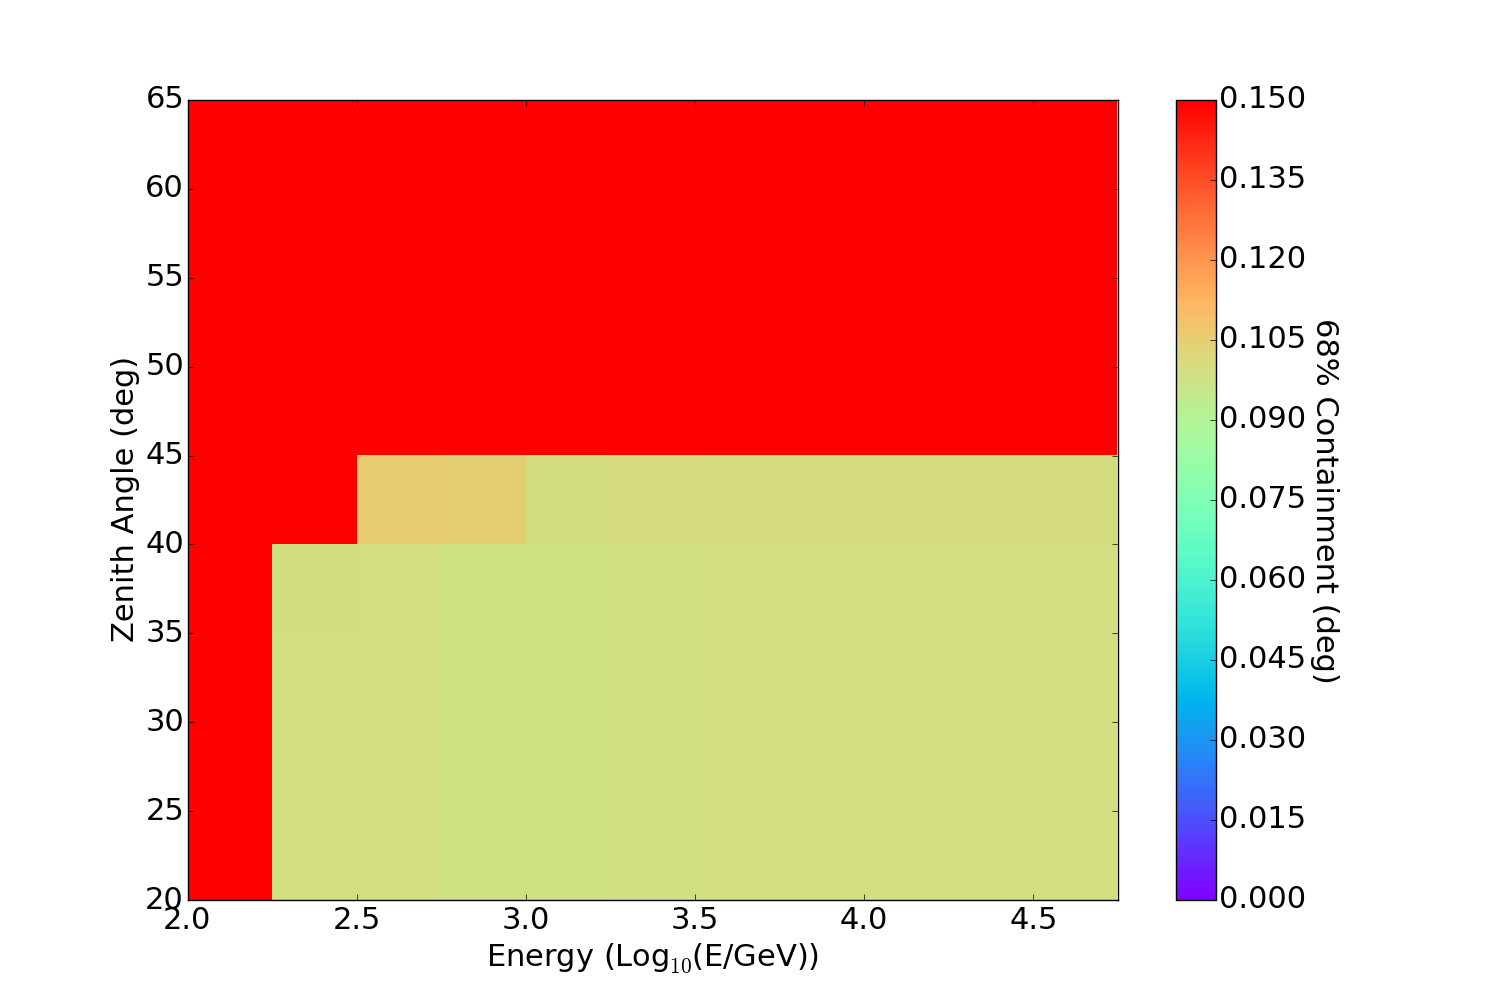
\includegraphics[width=0.47\linewidth]{PKS1510_rse.png}
      \label{fig:PKS1510_rse}
    }  
    \subfigure[Deviation from simulations.]{ 
      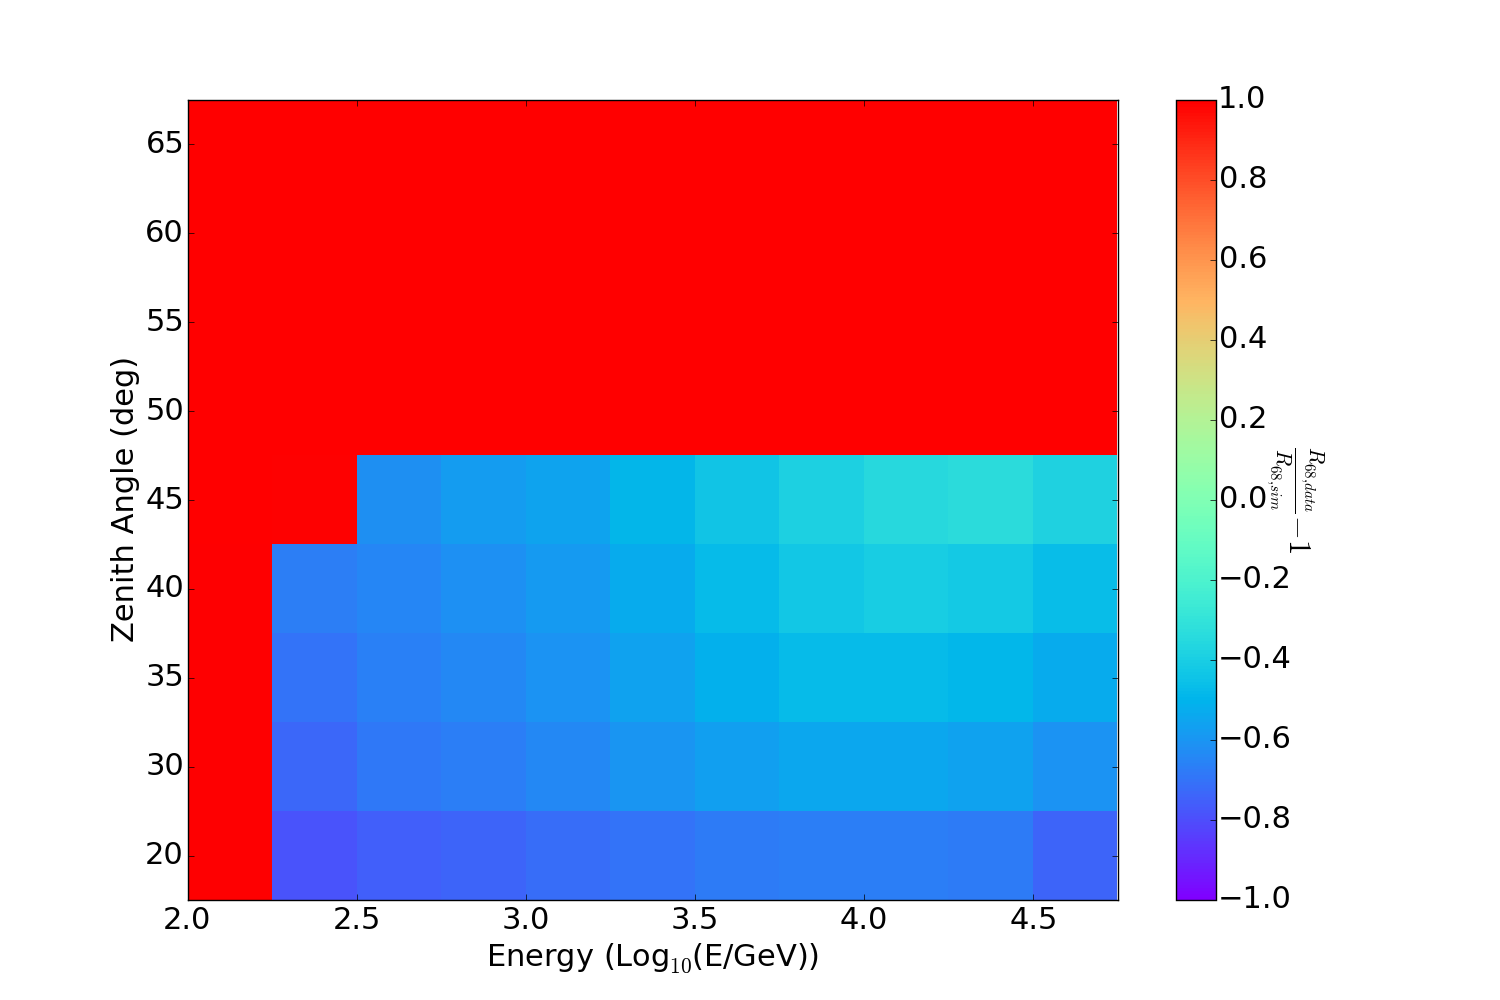
\includegraphics[width=0.47\linewidth]{PKS1510_sim.png}
      \label{fig:PKS1510_sim}
    }
    \subfigure[Number of events ($\log(N_{on}-\alpha N_{off})$).]{ 
      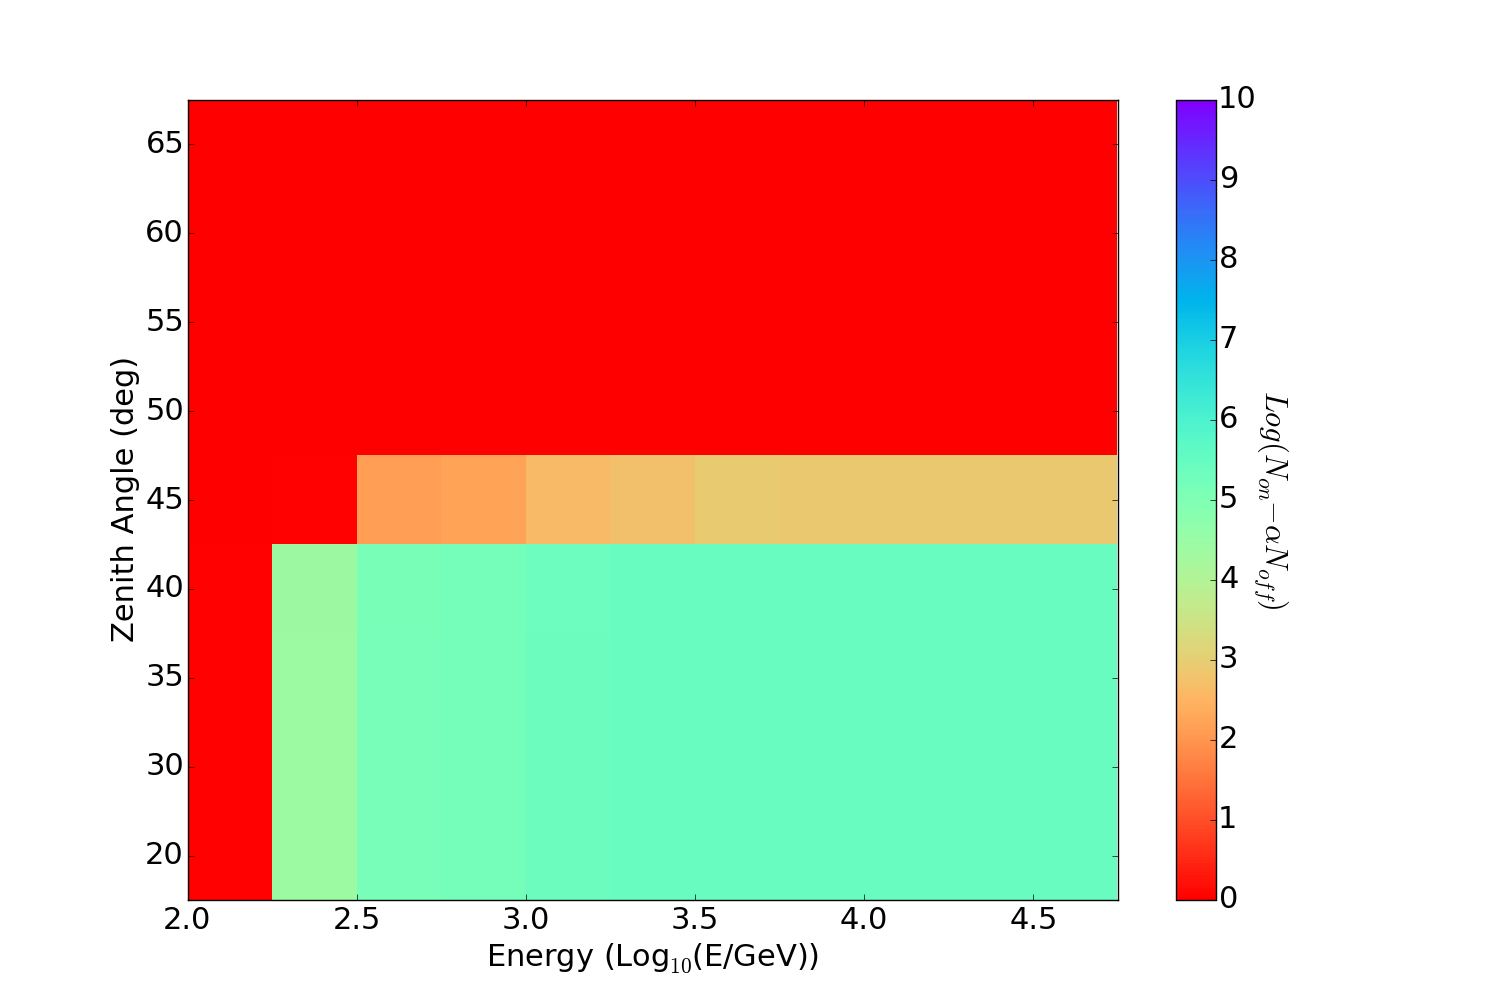
\includegraphics[width=0.47\linewidth]{PKS1510_Log_nevent.png}
      \label{fig:PKS1510_nevent}
    }  
    \subfigure[Li \& Ma significance.]{ 
      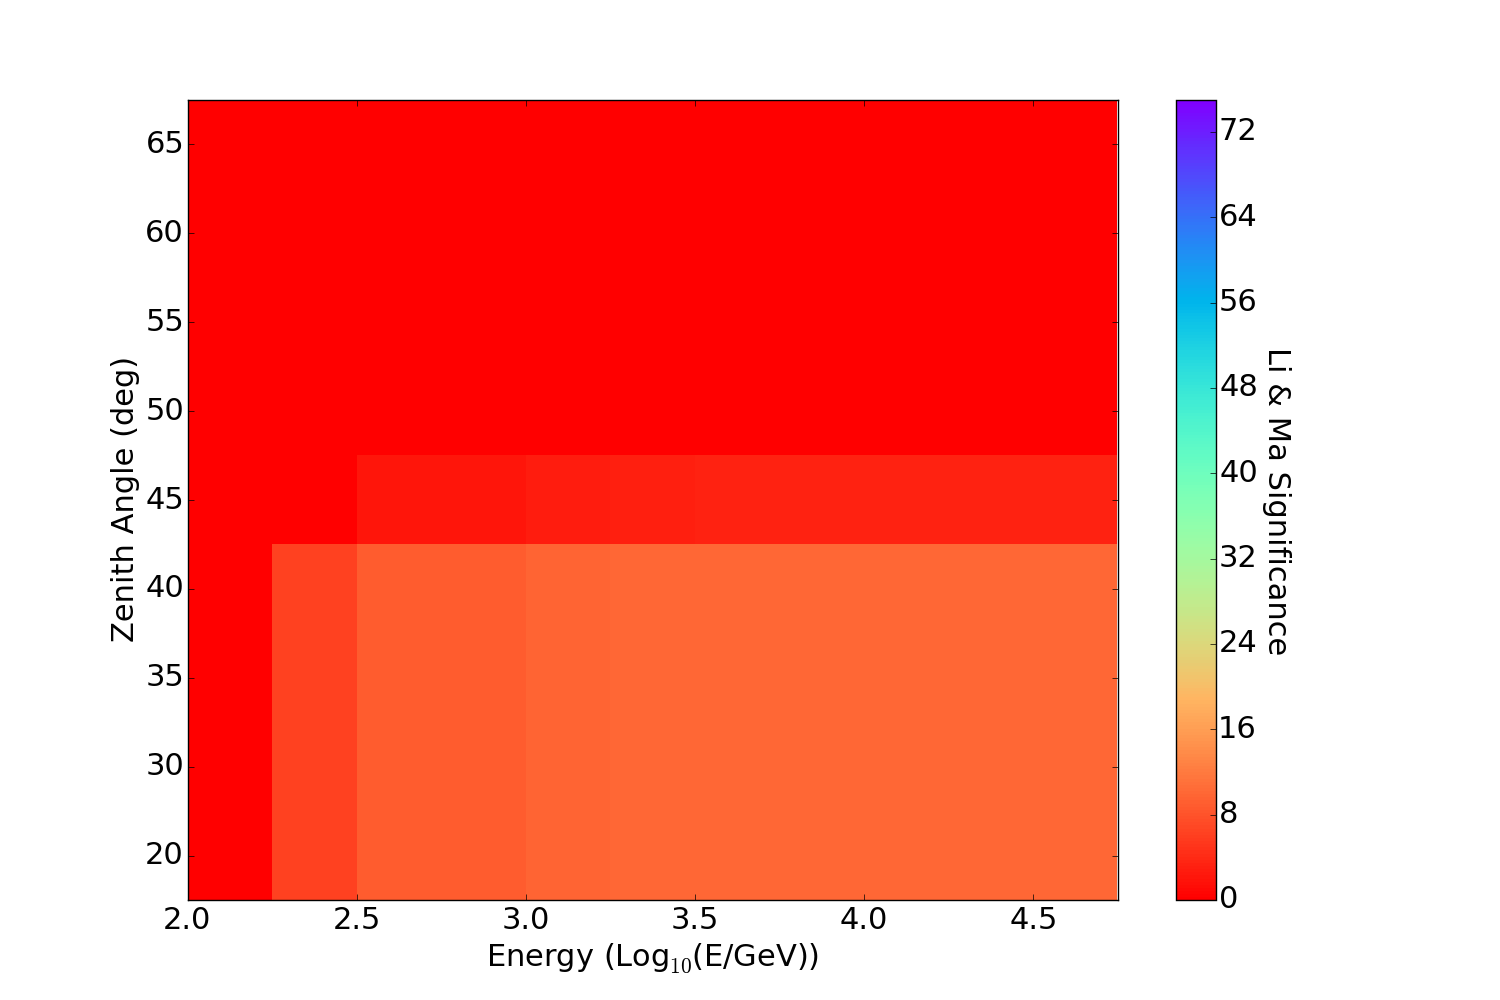
\includegraphics[width=0.47\linewidth]{PKS1510_LiMa.png}
      \label{fig:PKS1510_li_ma}
    }
  \end{center}
  \caption[PKS1510 direction reconstruction using Method5t.]{Reconstruction of the direction of PKS1510 using the new \disp tables.  In each case red denotes regions of no statistics.}
  \label{fig:PKS1510_disp}
\end{figure}

\end{document}
